\documentclass{config/PoliMi3i_thesis}
\usepackage{graphicx} % Required for inserting images
\usepackage{mathtools}
\usepackage{amssymb}
\usepackage[utf8]{inputenc} 
\usepackage{enumitem}
\usepackage{float}
\usepackage{multirow}
\usepackage{geometry}
\usepackage{multirow}
\usepackage{hyperref}
\usepackage{wrapfig}
\usepackage{lipsum}
\usepackage{longtable}
\usepackage{float}
\usepackage{array} 
\usepackage{enumitem} 
\geometry{margin=1in}
%\usepackage{adjustbox}
%\renewcommand{\arraystretch}{1.5}
\usepackage{longtable}
\usepackage[table]{xcolor}

\definecolor{bluepoli}{cmyk}{0.4,0.1,0,0.4}

% CONFIGURATIONS
\usepackage{parskip} % For paragraph layout
\usepackage{setspace} % For using single or double spacing
\usepackage{emptypage} % To insert empty pages
\usepackage{multicol} % To write in multiple columns (executive summary)
\setlength\columnsep{15pt} % Column separation in executive summary
\setlength\parindent{0pt} % Indentation
\raggedbottom 

% PACKAGES FOR LANGUAGE AND FONT
\usepackage[english]{babel} % The document is in English  
\usepackage[utf8]{inputenc} % UTF8 encoding
\usepackage[T1]{fontenc} % Font encoding
\usepackage[11pt]{moresize} % Big fonts

\newcommand\numfontsize{\@setfontsize\Huge{200}{60}}

% PACKAGES FOR TITLES
\usepackage{titlesec}
\usepackage{fancyhdr}
\fancyhf{}

% \titlespacing{\section}{left spacing}{before spacing}{after spacing}
\titlespacing{\section}{0pt}{3.3ex}{2ex}
\titlespacing{\subsection}{0pt}{3.3ex}{1.65ex}
\titlespacing{\subsubsection}{0pt}{3.3ex}{1ex}

% PACKAGES FOR ALGORITHMS (PSEUDO-CODE)
\usepackage{algorithm}
\usepackage{algorithmic}

% CONFIGURATIONS
\usepackage{parskip} % For paragraph layout
\usepackage{setspace} % For using single or double spacing
\usepackage{emptypage} % To insert empty pages
\usepackage{multicol} % To write in multiple columns (executive summary)
\setlength\columnsep{15pt} % Column separation in executive summary
\setlength{\parindent}{0pt} % Indentation
\raggedbottom
\setlength{\parskip}{1ex plus 0.5ex minus 0.2ex}

\usepackage{times}

% Title format: chapter
\titleformat{\chapter}[hang]{
\fontsize{50}{20}\selectfont\bfseries\filright}{\textcolor{bluepoli} \thechapter\hsp\hspace{2mm}\textcolor{bluepoli}{|  }\hsp}{0pt}{\huge\bfseries \textcolor{bluepoli}
}

% Title format: section
\titleformat{\section}
{\color{bluepoli}\normalfont\Large\bfseries}
{\color{bluepoli}\thesection.}{1em}{}

% Title format: subsection
\titleformat{\subsection}
{\color{bluepoli}\normalfont\large\bfseries}
{\color{bluepoli}\thesubsection.}{1em}{}

% Title format: subsubsection
\titleformat{\subsubsection}
{\color{bluepoli}\normalfont\large\bfseries}
{\color{bluepoli}\thesubsubsection.}{1em}{}

%For correctly numbering algorithms
\numberwithin{algorithm}{chapter}

% Shortening for setting no horizontal-spacing
\newcommand{\hsp}{\hspace{0pt}}
% TEXT SIZES:

%\Huge - Largest size
%\huge
%\LARGE
%\Large
%\large
%\normalsize - Normal/default size
%\small
%\footnotesize
%\scriptsize
%\tiny - Smallest size

%code setup
\usepackage{listings}
\usepackage{color}

\definecolor{dkgreen}{rgb}{0,0.6,0}
\definecolor{gray}{rgb}{0.5,0.5,0.5}
\definecolor{mauve}{rgb}{0.58,0,0.82}
\lstdefinelanguage{Alloy}{
    morekeywords={
        module, open, sig, abstract, extends, fact, pred, run, check, for, all, some, lone, one, no, implies, and, or, not, set, disj, in, fun, let
    },
    sensitive=true,
    morecomment=[l]{//},       % Commenti su una linea
    morecomment=[s]{/*}{*/},  % Commenti su più linee
    morestring=[b]",          % Stringhe fra doppi apici
}
\lstset{frame=tb,
  language=Alloy,
  aboveskip=3mm,
  belowskip=3mm,
  showstringspaces=false,
  columns=flexible,
  basicstyle={\small\ttfamily},
  numbers=none,
  numberstyle=\tiny\color{gray},
  keywordstyle=\color{blue},
  commentstyle=\color{dkgreen},
  stringstyle=\color{mauve},
  breaklines=true,
  breakatwhitespace=true,
  tabsize=3
}

\begin{document}

\fancypagestyle{plain}%
\fancyhf{} % Clear all header and footer fields
\fancyhead[RO,RE]{\thepage} %RO=right odd, RE=right even

\begin{titlepage}

\centering
{\bfseries\LARGE Software Engineering 2\\ 
\vskip0.2cm
}
 \large A.Y. 2024/2025


\vskip1.5cm



\includegraphics[width=10cm]{Images/logopoliazzurro.png}\centering
\vskip2cm

     
\centering
{\bfseries \Huge Students\&Companies\\
\vskip0.5cm
}
\huge Requirements Analysis and Specification Document\\
\vskip1.5cm
{\Large 
            Lo Presti Irene\\ 
            Lussana Matteo\\
}

\vskip2cm
\raggedright\large{
 Release date: 07/01/2025\\
 Version: 2.0}


\end{titlepage}

\pagebreak

\renewcommand*\contentsname{Table Of Contents}
\tableofcontents
%\pagenumbering{arabic}

\pagebreak
\chapter{Intro}
\section{Purpose}
The \textbf{S\&C system} is a platform designed to connect university students seeking \textbf{internships} with companies offering internship opportunities. The platform helps students and companies connect and use tools designed for their needs.\newline
\textbf{Students} are able to log in to the platform via their university credentials. Once they are logged in, they can \textbf{personalise their profile} by uploading their CV and inserting their skills, experiences and attitudes. They can \textbf{search for an internship} by using the search bar, or by waiting for personalised recommendations sent by the system. If they find a suitable internship, they can \textbf{contact} the company. They might also be contacted by a company, so they can accept or decline the offer. If a company accepts a student's application, the Selection Process begins, which involves an interview.\newline
\textbf{Companies} can publish \textbf{internship advertisements}, look actively for suitable candidates via the search bar or use the recommendations sent by the system. They can, as well, \textbf{contact students}, or they can accept or decline internship requests. They can \textbf{setup an interview} with possible candidates, and create customized forms for use during interviews linked to specific internship advertisements.\newline
Both students and companies can monitor the interactions regarding internships by the \textbf{Monitoring Section}. They can also provide \textbf{feedbacks} on their experiences with one another, whether after an interview or during an internship. These comments are published on the user’s profile.\newline
The \textbf{Recommendation Process} is based on an analysis by the system that considers the criteria used in the search bar by the student, the candidate profile inserted in the internship advertisement, and the feedback provided by both parties.
\subsection{Goals}
\begin{itemize}

    \item [\text{[G1]}] University students can find companies aligned with their interests, apply for internships, complete interviews, and track every stage of the process, from application to the successful completion of the internship.

    \item[\text{[G2]}] Companies can advertise their internship opportunities to find suitable students for the position, contact them, conduct interviews, hire the best candidates, and keep track of the entire process.

    %uniamo g2 e g3? g2 è un goal?
    %aggiungiamo i feedbacks???
    
\end{itemize}

\section{Scope}
\subsection{World Phenomena}

\begin{itemize}

    \item[\text{[WP1]}] University Students want to do an internship.

    \item[\text{[WP2]}] Companies offer internships to university students.

    \item[\text{[WP3]}] Companies are looking for students for internship positions.

    \item[\text{[WP4]}] University Students write their CV with their experiences, skills, and attitudes.

    \item[\text{[WP5]}] Companies decide the project (application domain, tasks to be performed, relevant adopted technologist, etc) and terms offered (salary, benefits, mentorship, etc).

    \item[\text{[WP6]}] Companies and potential candidates (students) establish a contract.

    \item[\text{[WP7]}] Companies do interviews with potential candidates.

    \item[\text{[WP8]}] University Students work as interns in the Companies.
    
\end{itemize}

\subsection{Shared Phenomena}
\subsubsection{World controlled}
\begin{itemize}
    \item [\text{[SP1]}] University Students create a profile and upload their CV.
    \item [\text{[SP2]}] Companies create a profile and the internship position.
    \item [\text{[SP3]}] Companies advertise the internship position.
    \item [\text{[SP4]}] University students look for an internship through the platform.
    \item [\text{[SP5]}] Students contact Companies they are interested in to initiate the process.
    \item [\text{[SP6]}] Companies contact Students who match their requirements to initiate the process.
    \item [\text{[SP7]}] Students and Companies can accept/refuse the offers made to them.
    \item [\text{[SP8]}] University Students and Companies provide feedback to S\&C.
\end{itemize}
\subsubsection{Machine controlled}
\begin{itemize}
    \item [\text{[SP9]}] S\&C platform informs Students when an internship they are interested in becomes available.
    \item [\text{[SP10]}] S\&C platform informs Companies about the availability of Students with CVs corresponding to their needs.
    \item [\text{[SP11]}] S\&C supports the selection process by helping Companies manage interviews and finalize the selection.
    \item [\text{[SP12]}] S\&C provides mechanisms to monitor the matchmaking process for both Students and Companies.
\end{itemize}

\section{Definitions, Acronyms, Abbreviations}
\subsection{Definitions}
\textbf{Single Sign-on} is an authentication method that allows users to log into multiple applications and websites using a single set of credentials. In the S\&C system, Students use their university credentials to log in.\newline
\textbf{Application Programming Interface} is a collection of functions and methods that allow the development of applications to interact with the features or data of an operating system, software, or other services.\newline
\textbf{RESTful APIs}: specific standadized architectural style for APIs.
\textbf{Web Socket}: computer communications protocol, providing a simultaneous two-way communication channel over a single Transmission Control Protocol (TCP) connection.
\textbf{Recommendation} is the process performed by the system that recommends to students potential internship positions that they might be interested in and to companies potential candidates.\newline
The \textbf{Chamber of Commerce Certificate} is an official document provided by the Chamber of Commerce that holds a legal certification value. It confirms the company's registration in the Business Register and includes its name, legal structure, and registration details.\newline
The \textbf{Revenue Agency} is a public entity that is not focused on profit but is dedicated to ensuring optimal tax compliance. Its primary responsibilities include collecting tax revenues, offering services and support to taxpayers, and conducting assessments and inspections to combat tax evasion.
\subsection{Acronyms}
ADV: advertisement\newline
SSO: Single Sign-on \newline
API: Application Programming Interface\newline
REST: Representational State Transfer\newline
HTTPS: HyperText Transfer Protocol Secure\newline
TLS: Transport Layer Security \newline
FCM: Firebase Cloud Messaging \newline
VAT number: value-added tax identification number (\textit {partita IVA})\newline
CEO: Chief Executive Officer \newline
HR: Human Resources\newline
CV: Curriculum Vitae
\subsection{Abbreviations}
G\#: Goal\newline
WP\#: World Phenomena\newline
SP\#: Shared Phenomena\newline
D\#: Domain Assumptions\newline
R\#: Functional Requirement\newline
UC\#: Use Case

\section{Revision History}
Version 1.0: 22/12/2024

\section{Reference Documents}
Specification document: Assignment RDD AY 2024-2025. \newline
Slides of the course "Software Engineering 2" held at Politecnico di Milano by Professor Rossi (a.y. 2024-25).\newline
Graduate Profile Survey 2022 by AlmaLaurea.\newline
Some definitions from the Definitions, Acronyms, Abbreviations section are taken from researches done on the Internet.\newline

\section{Document Structure}
\begin{enumerate}
    \item \textbf{Introduction}: this section includes a description of the system, done through the explanation of the \textbf{Purpose} of the system and the \textbf{Scope} of the problem that includes a list of \textbf{World and Shared Phenomena} concerning the project. There is also technical information to be able to read the document (\textbf{Definitions, Acronyms, Abbreviations}), the \textbf{Revision History}, the \textbf{Reference Documents}, and the \textbf{Document Structure}.
    \item \textbf{Overall Description}: a high-level explanation of how the platform works through the \textbf{Product prospective} section where there are the descriptions of some scenarios, the Domain Class Diagram and the State Diagrams, the \textbf{Product functions} that explain the most important requirements, the \textbf{User Characteristics} section, and the \textbf{Assumption, dependencies, and constraints} section that lists all the Domain Assumptions made to make the project work.
    \item \textbf{Specific Requirements}: detailed analysis of all the aspects shown in Chapter 2 to be used by the development team. This chapter includes the \textbf{External Interface Requirements}, the \textbf{Functional Requirements} explained through the Use Case paradigm, the \textbf{Performance Requirements}, the \textbf{Design Constraints}, and the \textbf{Software System Attributes}.
    \item \textbf{Formal Analysis using Alloy}: modelisation of the problem and formal check done using Alloy 6.
    \item \textbf{Effort Spent}: information about the time spent drafting the document divided per group members.
    \item \textbf{References}: this section lists the documents used to draft the project.
\end{enumerate}

\pagebreak
\chapter{Overall Description}
\section{Product perspective}
\subsection{Scenarios}
\textbf{Company signs up to the platform}\newline
The Company C wants to sign up to the S\&C platform, so a representative R opens the platform and clicks on the "Sign-up" button. The sign-up form is displayed, and R must provide the company's information as well as personal details to be correctly identified as a representative of C. To identify C, R enters the company's name, "C", VAT number, "IT 99999999999", and upload the Certificate of Registration from the Chamber of Commerce. To verify their own identity, R inserts their own company email, "rname.rsurname@companyc.com", and an authorisation letter signed by the CEO of C. 
After a couple of hours, R receives an email with a username for C, "company\_C\_123", and a link to setup a password. R clicks on the link and setup the new password. Now that the password is set, R is be able to log in to the platform, just like other colleagues working at Company C.
\newline\newline
\textbf{Student signs up to the platform and adds their personal information}
\newline
The Student S wants to sign up to the S\&C platform, so opens the platform and clicks on the "Sign-up" button. The sign up form is displayed, and S must provide the academic email, "sname.ssurname@univeristyu.com", and the university name, "University U". S1 is redirected to U's login page, here S1 can login. S1 returns to the S\&C platform Home Page. Now, the student S wants to upload their own personal CV and competences. So, S navigates to their personal page, clicks on "Upload new CV" and uploads the file with the drag and drop function. Then, to insert experiences, skills and attitudes on their profile, S clicks on 
"Insert new competence" and fills up the shown form:
\begin{itemize}
    \item New experience:
    \begin{itemize}
        \item Type (Skill, Experience, Attitude): "Skill"
        \item Name: "Coding"
        \item Description (optional): ""
    \end{itemize}
    \item New experience:
    \begin{itemize}
        \item Type (Skill, Experience, Attitude): "Skill"
        \item Name: "Team Working"
        \item Description (optional): ""
    \end{itemize}
    \item New experience:
    \begin{itemize}
        \item Type (Skill, Experience, Attitude): "Attitude"
        \item Name: "Confident"
        \item Description (optional): ""
    \end{itemize}
    \item New experience:
    \begin{itemize}
        \item Type (Skill, Experience, Attitude): "Experience"
        \item Name: "Internship at ABC Company"
        \item Description (optional): ""
    \end{itemize}
\end{itemize}
When finished, S clicks on the "Done" button and is redirected on the profile page where the new competences are shown.
\newline\newline
\textbf{Company creates an advertisement for an internship position along with the corresponding interview form.}\newline
A representative, R, of a Company C, who is logged in the S\&C platform, wants to create an advertisement for a new internship position available in C. R navigates to the Profile section and clicks on the "Create New Internship Advertisement" button. R is presented with a form where they must provide all relevant details about the internship, so R inserts:
\begin{itemize}
    \item Name of the internship position: "Optimization of delivery transport lines to newsstands"
    \item Location: "Milan"
    \item Candidate's profile: "Management Engineering, Computer Engineering, Mobility Engineering students. Technical skills: data analysis, operational flow analysis, and basic programming with the creation of software for project management. Personal skills: aptitude for working in a Small and Medium-sized Enterprise. Spoken languages: Italian (mandatory) and English"
    \item Project description:
    \begin{itemize}
        \item Educational objectives: "Operation in a multifunctional work environment and ability to analyze and execute a project"
        \item Skills to be acquired: "Fleet analysis, route scheduling, and time slot management"
    \end{itemize}
    \item Terms offered:
    \begin{itemize}
        \item Employment Type: "Full-time (40 hours per week)"
        \item Duration: "4 months"
        \item Total Duration in Hours: "420 hours"
        \item Open Positions: "1"
        \item Travel Requirements: "No"
        \item Benefits: "Networking opportunities within the industry and meal vouchers or subsidized meals"
    \end{itemize}
\end{itemize}
R clicks on the "Done" button, now the new advertisement is published on the platform, and R is redirected to the advertisement page.
R also wants to create the form to be compiled during the interviews for this position. So, R clicks on the button "New Interview Form", and inserts in the presented form all the aspect that are needed to be evaluated during the interview as well as the evaluation methods (e.g., scoring from 1 to 5, written comments):

\begin{itemize}
    \item Name
    \item Surname
    \item Date
    \item Interviewer
    \item General Information (evaluated with "Excellent", "Good", "Satisfactory", "Needs Improvement"):
    \begin{itemize}
        \item Punctuality
        \item Appearance/Professionalism
        \item Communication Skills
    \end{itemize}
    \item Skills and Qualifications:
    \begin{itemize}
        \item Educational Background ("Meets requirements", "Exceeds requirements", "Below requirements")
        \item Relevant Work Experience ("Extensive", "Sufficient", "Limited", "None")
        \item Technical Skills ("Extensive", "Sufficient", "Limited", "None")
        \item Problem-Solving Ability ("Excellent", "Good", "Satisfactory", "Needs Improvement") 
    \end{itemize}
    \item Behavioral Traits (evaluated with "Excellent", "Good", "Satisfactory", "Needs Improvement"):
    \begin{itemize}
        \item Teamwork and Collaboration
        \item Adaptability
        \item Initiative
    \end{itemize}
    \item Job-Specific Questions (evaluated with "Excellent", "Good", "Satisfactory", "Needs Improvement"):
    \begin{itemize}
        \item Knowledge of the Field/Industry
        \item Understanding of the Role
        \item Interest in the Position/Company
    \end{itemize}
    \item Overall Assessment:
    \begin{itemize}
        \item Strengths
        \item Areas for Improvement
        \item Recommendation ("Strongly Recommend", "Recommend", "Recommend with Reservations", "Do Not Recommend")
        \item Additional Comments
    \end{itemize}
\end{itemize}
R clicks on the "Submit" button, so the form is created and available on the ADV page. 
\newline\newline
\textbf{Student looks for an internship and send a request}
\newline
Student S wants to find an internship to enhance their personal career, so, from the homepage, S clicks on the research bar and types the desired characteristics of the internship: "Milan, full-time, paid over 2000€" and presses "Enter". The System shows an alert: there are no results. So, S deletes the characteristics and writes "Milan, full-time". The system shows the correspondent internships, 15 in this case. The student press on the first showed internship in order to visualize the ADV page: it is not in line with S's interests. So, S goes back with the "back arrow" and presses on the second showed internship. S reads the internship's advertise and then clicks on the company's name to visit its page. S approves this internship, so goes back to the internship ADV and presses the "Contact" button to send a request. S add an optional message: "Dear Company C, I am a business management student with a strong interest in marketing strategies, eager to apply my skills and gain hands-on experience. I would be thrilled to contribute to your team as an intern and further develop my expertise. Thank you for considering my application. Best regards, S1."
\newline\newline
\textbf{Student consults a recommendation and send a request}
\newline
Student S wants to check their personal inbox, S notice that they received a recommendation in line with their skills and attitudes. S consults the recommendation about a Company C and clicks on the "Contact" button to send a request, a window opens asking if S wants to add a message, S selects "No". Then S clicks on the Monitor icon and the System shows the monitor view where S can visualize the current state of their request.
\newline\newline
\textbf{Company manages internship requests}\newline
A representative, R, of a Company C, who is logged in the S\&C platform, wants to respond to internship requests received. C navigates to the Inbox Section and opens a message from Student S1. R reads the message and decides to visit S1's personal profile, so R clicks on S1's name and is redirected to their profile. R approves S1 as a potential candidate for the internship, so R clicks on the "Back" button to go back to S1's request and clicks on the "Accept" button. A window opens asking if R also wants to setup a date for the interview. R clicks on the "Setup interview" button and fills out the form with possible date and time slots:
\begin{itemize}
    \item Tuesday, December 10, from 10:00 AM to 11:00 AM or from 11:00 AM to 12:00 PM
    \item Thursday, December 12, from 2:00 PM to 3:00 PM or from 3:00 PM to 4:00 PM
\end{itemize}
When R finishes, they press "Send" and the message is sent to S1. 
R then returns to the Inbox Section and selects another message from Student S2. S2 is not suitable for Company C, so R clicks on the "Reject" button. A windows opens asking if R wants to add a message. R clicks on "Write Message" and writes a few lines to S2 explaining the reasons behind the decision: "Dear S2, thank you for your application for the internship position. After careful consideration, we regret to inform you that we have decided to move forward with other candidates whose qualifications more closely match the requirements for this role. We appreciate the time and effort you invested in your application and encourage you to apply for future opportunities.
Best regards,
R, HR representative", then clicks on "Send".
\newline\newline
\textbf{Student consults an internship request from a Company, consult the offer and the company profile and reject the offer}
\newline
Student S, who is attending an internship at a Company C1, checks their personal inbox and notices that has received a request from a Company C2. S consults the advertise and notice that the proposed internship period is not compatible with the current internship that they are attending. Anyway S decides to have a look of the Company page so press the company name and the System shows the Company Profile. Then S decides that the company is in line with their own interests so goes back to the advertise page clicking the back arrow and presses the "reject" button and writes a short message: "Thank you for the offer, unfortunately, during the period that you proposed I am busy with another company, so I have to reject your propose. However, I really appreciate your company and your work, so do not hesitate to contact me if you have other offers, best wishes, S".
\newline\newline
\textbf{Company writes feedbacks}
\newline
A representative, R, of a Company C, who is logged in the S\&C platform, wants to write some feedbacks regarding two Students S1 and S2. S1 did an interview for C that went well. However, C decided to go in another direction. R wants to write a positive feedback for S1, so R navigates to the Monitor Section, selects the internship position S1 was applying for, and press the "Feedback" button next to S1's name. R fills out the form presented:
\begin{itemize}
    \item \textbf{Leave an optional comment (it will be displayed on the Student personal page):} "C appreciates your time and preparation for the interview. Although you were not selected, your professionalism and potential stood out. Wishing you success in your future opportunities!"
    \item \textbf{Answer the following questions regarding the student's profile to help make better recommendations} (these answers will only be used by the S\&C system and will not be displayed anywhere):
    \begin{itemize}
        \item \textbf{Are the competences displayed on the student's profile consistent with their actual abilities?} (Yes, No, Not checked):
        \begin{itemize}
            \item Coding skills: "Yes"
            \item English C1: "Not checked"
            \item Effective communication: "Yes"
            \item Proactive Mindset: "Not checked"
            \item Team-Oriented: "Not checked"
        \end{itemize}
        \item \textbf{Is the CV consistent with the student's actual experiences?}: "No"
        \item Please explain why the CV is not consistent: "The student did not work part-time at Company ABC in Milan"
    \end{itemize}
    \item\textbf{Answer the following questions regarding the impression received during the interview with a number between 1 (Needs Improvement) to 4 (Accomplished)}:
    \begin{itemize}
        \item Punctuality 
        \item Communication Skills
        \item Critical Thinking Skills
        \item Confidence and Poise
        \item Knowledge of the Company
        \item Enthusiasm for the Role
    \end{itemize}
\end{itemize}

R writes the comment about S1 and presses "Submit". The comment will appear on S1's personal page.
On the other hand, Student S2 did a brief internship, but C is not satisfied with S2's behavior. To write feedback about S2, R navigates to the Monitoring Section and then to the Students Employed section, clicks on S2's name, and select "Feedback".  R fills out the form presented:
\begin{itemize}
    \item \textbf{Leave an optional comment (it will be displayed on the Student personal page):} "We had the opportunity to host S2 for a brief internship at C. During this time, we observed some challenges in punctuality, as consistent tardiness impacted daily productivity. Additionally, while S2 presented a skill set on their CV, these skills did not align with the expectations required for the role. We encourage S2 to focus on enhancing time management and further developing the skills highlighted in their resume to meet the demands of future opportunities. We believe in the potential for growth and improvement through constructive feedback and continued effort. Best wishes for future endeavors."
    \item \textbf{Answer the following questions regarding the student's profile to help make better recommendations} (these answers will only be used by the S\&C system and will not be displayed anywhere):
    \begin{itemize}
        \item \textbf{Are the competences displayed on the student's profile consistent with their actual abilities?} (Yes, No, Not checked):
        \begin{itemize}
            \item Data analysis and visualization: "No"
            \item Project management tools : "Yes"
            \item Time management: "No"
            \item Adaptability: "Yes"
        \end{itemize}
        \item \textbf{Is the CV consistent with the student's actual experiences?}: "No"
        \item Please explain why the CV is not consistent: "Competences described above."
    \end{itemize}
    \item\textbf{Answer the following questions regarding the impression received during the internship with a number between 1 (Needs Improvement) to 4 (Accomplished)}:
    \begin{itemize}
        \item Punctuality 
        \item Communication Skills
        \item Critical Thinking Skills
        \item Confidence and Poise
        \item Ability to Handle Stress
        \item Team Collaboration 
        \item Enthusiasm for the Role
    \end{itemize}
\end{itemize}
The comment will appear on S2's personal page.

\subsection{Domain Class Diagram}
\begin{figure}[H]
    \centering
    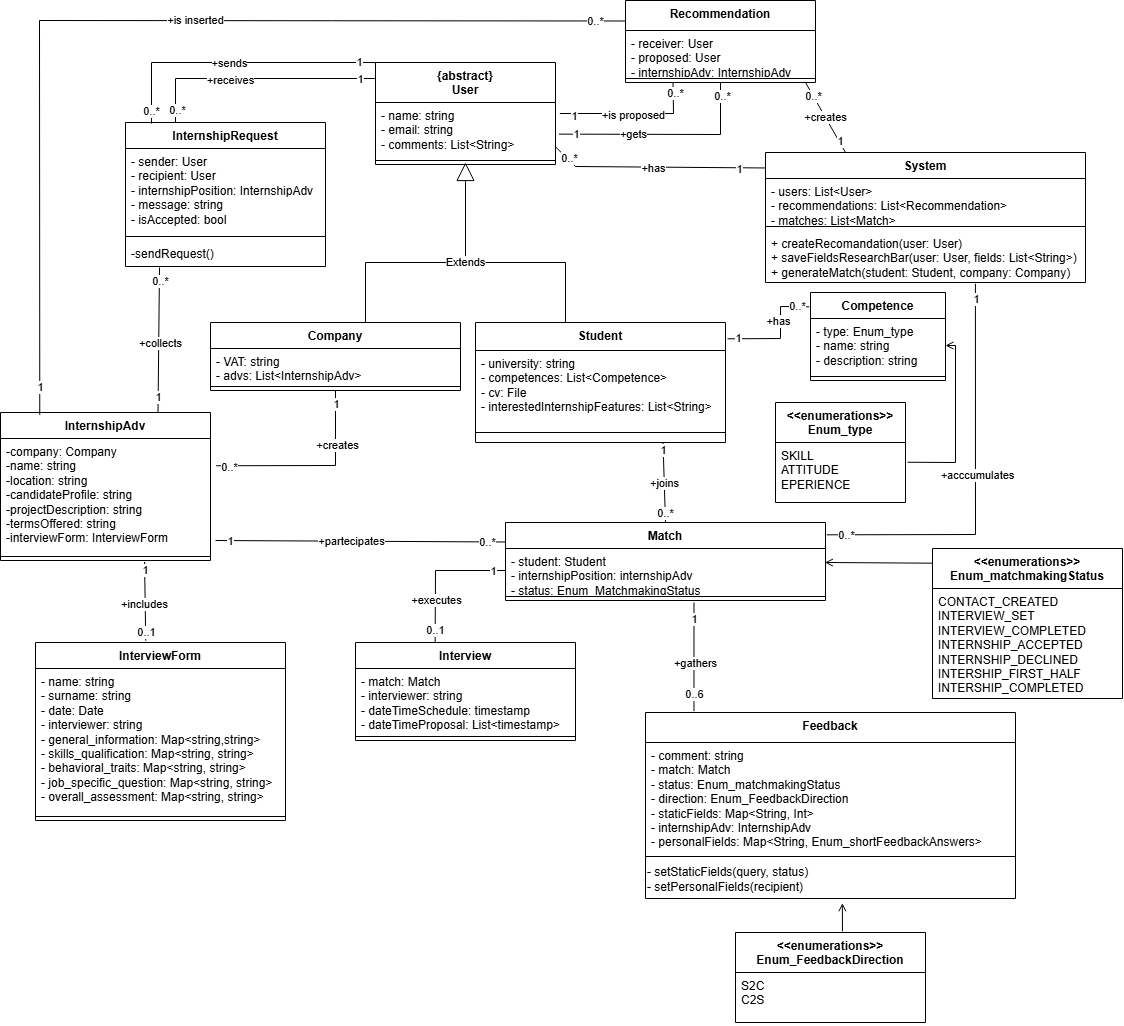
\includegraphics[width=15cm]{Images/RASD-Final Domain Class Diagram.png}
    \caption{UML Domain Class Diagram}
\end{figure}
This Domain Class Diagram shows all the classes that will be created to manage the system and the relations between them. Only the relevant methods are present.
Here follows a more detailed explanation of the classes and the relations.\newline
The class \textbf{System} manages the users, creates the recommendations (represented by the class \textbf{Recommendation}), and handles the matches between students and internship positions. The abstract class \textbf{User} is created to generalise the two types of user that navigate through the system: Student and Company. \textbf{Student} is the class dedicated to university students, in particular, it has a list of \textbf{Competence}s, each one of them can be one of three types (\textbf{Skill}, \textbf{Attitude}, \textbf{Experience}) and has a description. The list called \textbf{interestedIntenshipFeatures} contains the fileds inserted in the search bar by the student, they are used by the System to create appropriate recommendations. \textbf{Company} handles the profile of a company, it is linked to the \textbf{InternshipAdv} class that manages the internship advertisements. This class contains all the relevant information that will be shown in the ADV, in particular it contains the field \textbf{candidateProfile} that will be used by the System to make consistent recommendation. It also includes the \textbf{InterviewForm} that contains all the information that has to be inserted in the form to be used during the interview for the advertised internship position. It can be inserted after a while from the creation of the ADV, so, for this reason, the cardinality is 0 to 1.\newline
The class \textbf{InternshipRequest} represent the request sent by the company (or the student) to the student (or the company) regarding a specific internship ADV. The boolean \textbf{isAccepted} will turn true if the counterpart accepts the propose. \newline
When a contact is made then a match between the student and the ADV is created. This is handeld by the class \textbf{Match} with the field \textbf{matchmakingStatus} that keeps track of the status of the match, it goes from the setting of the interview to the completion of the internship. It has a relation ("executes") with the class \textbf{Interview} that contains the information relevant for the interview between that specific Match. The class Match is also related to the class \textbf{Feedback}. A feedback can be created only in specific states of the match: after the interview is terminated ({INTERVIEW\_COMPLETED}), at the first half of the internship ({INTERNSHIP\_FIRST\_HALF}) and at the end ({INTERNSHIP\_COMPLETED}). Drafting the feedback is optional, and can be done in both directions: by the student for the company (S2C) and by the company for the student (C2S). This explains the cardinality 0 (it is optional) to 6 both the student and the company answer to all the feedback of the three states). 

\subsection{State Diagrams}
\textbf{Sign up and Login}\newline
\begin{figure}[H]
    \centering
    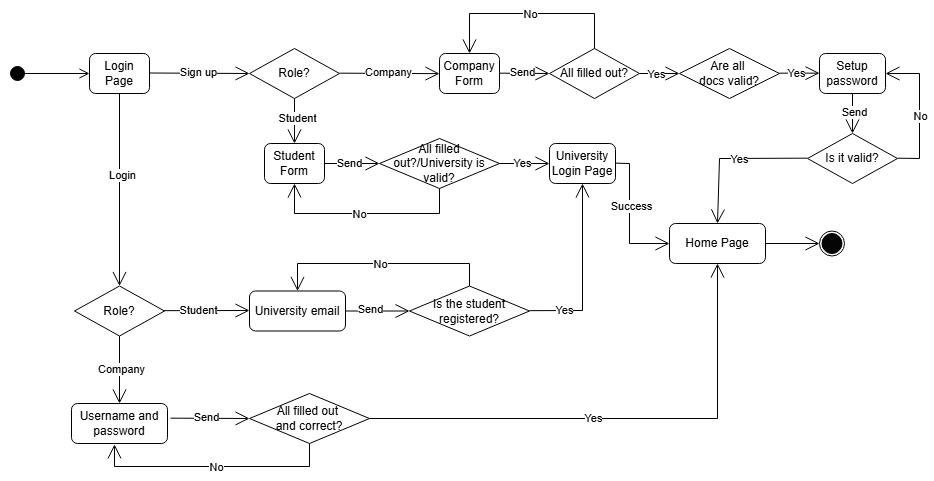
\includegraphics[width=15cm]{Images/State_Diagrams/RASD-SD-login_signup.drawio.png}
    \caption{Sign up and Login State Diagram}
\end{figure}
This State Diagram describes the processes of Sign Up and Login for both Companies and Students. 
\newline

\textbf{Update Student's Profile}\newline
\begin{figure}[H]
    \centering
    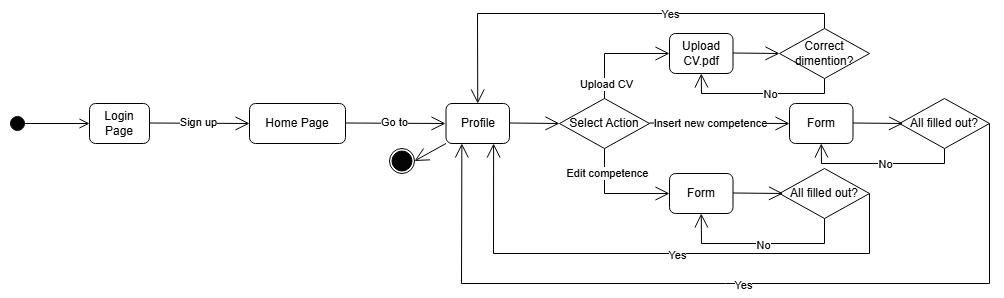
\includegraphics[width=15cm]{Images/State_Diagrams/RASD-SD-Update student profile.drawio.png}
    \caption{Update Student's Profile State Diagram}
\end{figure}
This diagram illustrates how a Student can updates their profile. The Login step is implicit because it is shown in the first diagram. The Student can upload a new CV, insert new competences, or edit the ones already present. 
\newline

\textbf{Creation of an Internship Advertisement}\newline
\begin{figure}[H]
    \centering
    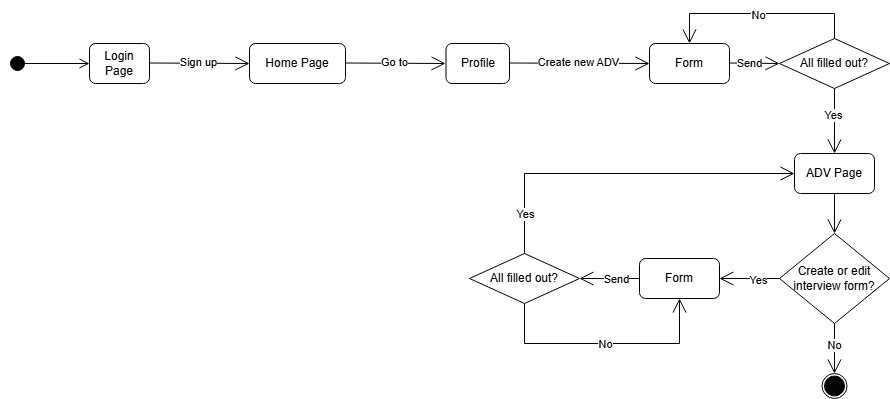
\includegraphics[width=15cm]{Images/State_Diagrams/RASD-SD-create adv.drawio.png}
    \caption{Creation of an Internship Advertisement State Diagram}
\end{figure}
This graph shows the process of the creation of an Internship Advertisement done by a Company. As before, the Login step is implicit. The Company can also decide whether to create the Interview Form immediately.
\newline

\textbf{Company's Matchmaking Process}\newline
\begin{figure}[H]
    \centering
    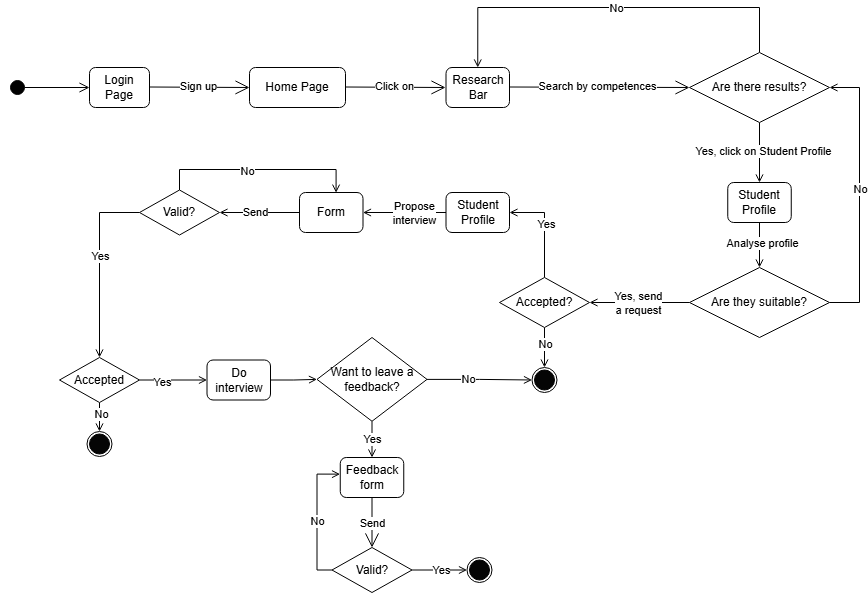
\includegraphics[width=15cm]{Images/State_Diagrams/RASD-SD-Matchmaking.drawio.png}
    \caption{Company's Matchmaking Process State Diagram}
\end{figure}
This State Diagram describes the process that a Company has to go through in order to search for a candidate, contact them and set up an interview. The Login step is implicit.
\newline

\textbf{Feedback}\newline
\begin{figure}[H]
    \centering
    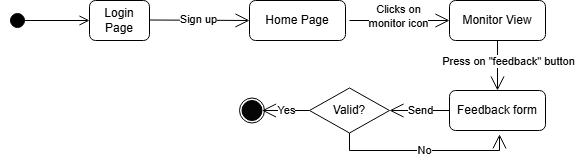
\includegraphics[width=15cm]{Images/State_Diagrams/RASD-SD-Feedback.drawio.png}
    \caption{Feedback State Diagram}
\end{figure}
This State Diagram shows how a User can leave a feedback. The Login step is implicit and it is assumed that the user has matches.
\newline

\section{Product functions}
\textbf{Sign up and Login}\newline
The S\&C platform allows users to register and log in depending on their role. Students can manage both the sign up and log in through their university credentials, i.e. the system redirects them to their university's website. A representative of a Company can register it by filling a form where they have to identify both the company and themselves. To identify the Company, they have to insert the VAT number and upload a certificate of registration at the Chamber of Commerce. To identify themselves, they have to insert their own company email and upload a letter of authorisation or official assignment signed by the CEO or an HR referent. The uploaded documentation will be reviewed by S\&C employees and if everything is correct, an email will be sent to the representative containing a username and a link to set a password.

\textbf{Update Student's profile}\newline
Students can update their profile in many ways: they can upload their CV (as a pdf) for the first time, but also upload a new version if they have updated it. They can also insert personal competences (such as skills, experiences, and attitudes) to be shown in their profile. Such competences can be modified and/or deleted whenever they want.

\textbf{Create internship's advertise}\newline
The platform allows representatives of Companies to create internship advertises where they can specify the project of the internship, the profile of the candidate they are looking for, and the terms offered. These advs can be modified or deleted from the platform.

\textbf{Proactive Research}\newline
The platform allows users to use a search bar. Students can find internships by inserting specific requirements about the project and/or the teams offered. If the system finds some suitable internships, it shows them to the Student who can click on them to visualise the adv and/on the Company's profile and eventually contact them. Companies' representatives can search for suitable candidates through this search bar by inserting the competences they are looking for. If the system finds Some suitable candidates, it shows them to the representative who can click on them to visualise the Student's profile and eventually contact them. 

\textbf{Recommendation}\newline
S\&C notifies users about potential matches. Proactive research criteria provided by students are used to recommend suitable internship opportunities. Similarly, the candidate profile specified in an internship advertisement is used to recommend matching students to companies. Recommendations are also based on the feedbacks received by the users. These recommendations are shared with the users and can be accessed via the Inbox section present in their profile. From the recommendation notifications, students can explore the internship advertisement and the company's profile, while companies can view the students' profiles.

\textbf{Matching between company and student and establishment of a cost }\newline
S\&C allows Student to contact Company that find on the platform through the research bar or thanks to the recommendation. S\&C also allows Company to contact Student that they found by the research bar or thanks to the recommendation. The system also will inform the Students and Companies if someone wants to contact them, the user contacted will see a message in the inbox section, and thorough that they will be able to get information about the user who contacted them. When receiving a message, the user can decide to reject the offer or to establish a contact.

\textbf{Selection process}\newline
S\&C allows Company, after they establish a contact with a student, to propose to the student some Date and Time slots in order to schedule an interview, the student will be pale to accept one of the proposals or reject them all. The system will provider assistance to Company during the interview too, indeed S\&C allows Company to create a standard form where they can write all the aspects that the interviewer will evaluate during the meeting.

\textbf{Feedback}\newline
S\&C allows Students to leave a feedback about the Company or some aspect of a Company during the selection period or about the internship that they are attending or have just finished. And allows Company to write feedback about a Student after the review, during the internship, or when the internship is just finished. The platform will use this feedback to enhance its recommendation system.

\textbf{Monitoring of the matchmaking process}\newline
S\&C allows every user to monitor their situation, in particular help to understand in which state of matchmaking or internship the users are. For Company S\&C allows to monitor the state of every student that is in contact with and with the ones who are attending an internship in the company, allowing us to leave a feedback to them. For Student allows to monitor the state of the matchmaking with the companies or the state of the internship that their are attending.

\section{User Characteristics}. Users who can interact with the system can be subdivided into two groups:
\begin{enumerate}
    \item University students seeking an internship related to their field of study. 
    \item Companies looking for university students with specific qualifications to fill internship positions.
\end{enumerate}



\section{Assumption, dependencies, and constraints}
\begin{itemize}
    \item[\text{[D1]}] Companies offer real internship positions.
    \item[\text{[D2]}] Students search for internship related to their course.
    \item[\text{[D3]}] Students write their own CV according to their real experiences, skills, and attitudes.
    \item[\text{[D4]}] The experiences, skills, and attitudes shown in the students' profiles are consistent with those in their respective CVs.
    \item[\text{[D5]}] Companies are honest in listing the projects and the terms offered.
    \item[\text{[D6]}] Students and companies are honest when giving feedbacks.
    \item[\text{[D7]}] Students and companies have access to a working Internet connection.
    \item[\text{[D8]}] Employees of the S\&C platform that checks the validity of a Company are capable and honest.
\end{itemize}


\pagebreak
\chapter{Specific Requirements}
\section{External Interface Requirements}
\subsection{User Interfaces}
The S\&C user interfaces will consist of a website and a mobile application. The website will primarily be used by companies and students, e.g., to upload their CVs and edit their profiles. The mobile application, however, will be particularly useful for students who want to quickly check their inbox or monitor section. At least one interface will be accessible to anyone with an Internet connection and a compatible device.
\subsection{Hardware Interfaces}
For hardware interfaces, users can choose between a computer (with a browser) or a mobile device, such as a smartphone or tablet, with the mobile application installed. Every device will have to be connected to the Internet.
\subsection{Software Interfaces}
The system requires the Revenue Agency's API to verify the validity of a company's data. It also uses universities' SSO to manage student login. Additionally, it includes an admin dashboard for reviewing company registrations, responding via email, and monitoring user feedback.
\subsection{Communication Interface}
The platform ensures secure and efficient communication through a combination of protocols. HTTPS encrypts all data transmitted between clients and servers, ensuring confidentiality and integrity. RESTful APIs are used to integrate with external systems such as the Revenue Agency and university SSO. Secure messaging is achieved through WebSocket connections encrypted with TLS, enabling real-time communication. Finally, Firebase Cloud Messaging (FCM) ensures reliable push notifications to mobile devices.
\section{Functional Requirements}

\textbf{Sign up and Log in}
\begin{itemize}
    \item[\text{[R1]}] S\&C allows Students to sign up to the platform through their university credentials using SSO access.
    \item[\text{[R2]}] S\&C allows Student to login via their university credentials.
    \item[\text{[R3]}] S\&C allows Companies to sign up to the platform by asking the representative of the company to insert their company email, the VAT number of the company, a Certificate of registration at the Chamber of Commerce, and a letter of authorisation or official assignment signed by a CEO or a HR referent. They have to choose a password.
    \item[\text{[R4]}] S\&C allows Companies to login to the platform via password and username (created by the system).
    
\end{itemize}

\textbf{Update Student's profile}
\begin{itemize}
    \item[\text{[R5]}] S\&C allows Students to upload the PDF of their CV (both for the first time and other times if there have been some changes).
    \item[\text{[R6]}] S\&C allows Students to insert new experiences, skills, and attitudes on their profile.
    \item[\text{[R7]}] S\&C allows Students to edit or delete experiences, skills, and attitudes present on their profile.
\end{itemize}

\textbf{Create internship's advertisement}
\begin{itemize}
    \item[\text{[R8]}] S\&C allows Companies to create an advertisement regarding an internship position they are offering, explaining the project of the internship and the terms offered.

    \item[\text{[R9]}] S\&C allows Companies to modify and remove an advertisement posted on their page.
\end{itemize}

\textbf{Proactive research}
\begin{itemize}
    \item[\text{[R10]}] S\&C allows Students to use a research bar to find appropriate internship positions by inserting specific requirements about the project and/or the terms offered.
    
    \item[\text{[R11]}] S\&C allows Companies to use a research bar to find appropriate candidates for their internship positions by inserting specific experiences, skills and/or attitudes the candidates should have.
\end{itemize}

\textbf{Recommendation}
\begin{itemize}
    \item [\text{[R12]}] S\&C informs students when an internship that might interest them becomes available.

    \item [\text{[R13]}] S\&C informs companies about the availability of a student whose CV corresponds to their needs.
\end{itemize}

\textbf{Matchmaking between company and student and establishment of a contact}
\begin{itemize}
    \item [\text{[R14]}] S\&C allows Students to contact a company they are interested in.
    
    \item [\text{[R15]}] S\&C allows Companies to contact Students they are interested in.

    \item [\text{[R16]}] S\&C informs a Student when a Company shows interest in their profile by sending the Student the Company's offer. The Student can accept or decline the offer.

    \item [\text{[R17]}] S\&C informs a Company when a Student shows interest in its offer by sending to the Company the Student's CV, the Company can accept or decline the offer.

    \item [\text{[R18]}] S\&C communicates to Students or Companies if their requests are successful.
\end{itemize}

\textbf{Selection process}
\begin{itemize}
    \item [\text{[R19]}] S\&C allows Companies to setup an interview with the candidates.

    \item [\text{[R20]}] S\&C allows Companies to write a form with all the aspects that will be considered during the interviews.

    \item [\text{[R21]}] S\&C allows Companies to modify or delete the interview form created.

    \item [\text{[R22]}] S\&C allows Companies fill the form during the interview.
\end{itemize}

\textbf{Feedback}
\begin{itemize}
    \item [\text{[R23]}] S\&C allows Students to give personal feedback during the selection period about the Company's selection method or during the internship period about the internship itself.

    \item [\text{[R24]}] S\&C allows Companies to give feedback after the interview or during the internship about a single Student.
\end{itemize}

\textbf{Monitoring of the matchmaking process}
\begin{itemize}
    \item [\text{[R25]}] S\&C offers Students the possibility to monitor their matchmaking process with a Company (state of the matchmaking, scheduled interview, interview results).

    \item [\text{[R26]}] S\&C offers Companies the possibility to monitor their matchmaking process with a Student.

    \item [\text{[R27]}] S\&C offers Students and Companies the possibility to monitor the state of the internship.
\end{itemize}

\subsection{Use Case Diagram}

\begin{figure}[H]
    \centering
    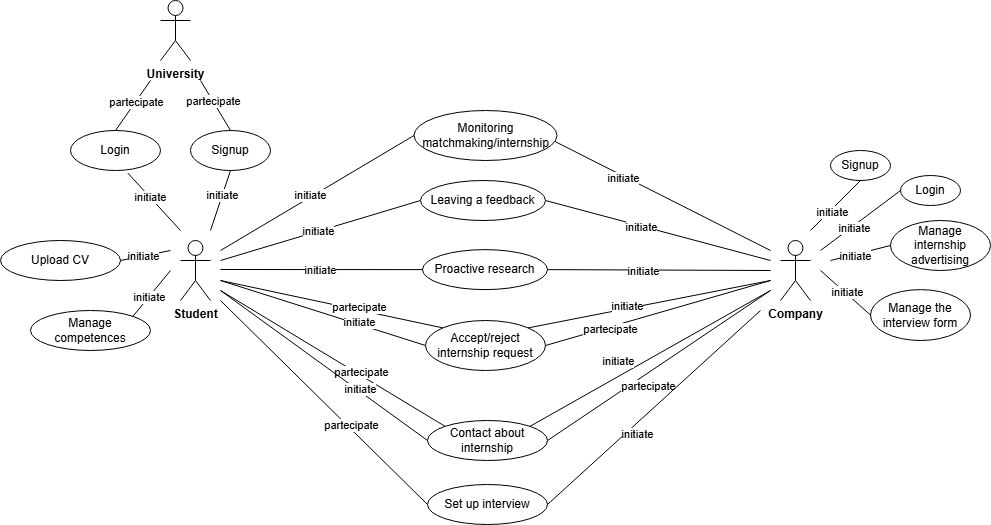
\includegraphics[width=15cm]{Images/usecasediagram2.png}
    \caption{Use Case Diagram}
\end{figure}

\subsection{Use Cases}

% Contatore
\newcounter{useCasesCounter}

\newcommand{\nextUseCases}{\stepcounter{useCasesCounter}\arabic{useCasesCounter}}

\textbf{[UC\nextUseCases] Students Signup}
\begin{table}[H] %per metterla esattamente dopo il titoletto
    \centering
    \begin{tabular}{|p{3cm}|p{10cm}|} 
    \hline
    Name & Students Sign up \\ \hline
    Actor  & Student, University website\\ \hline
    Entry Condition  & A university student wants to use the platform, they are in the login page but they are not registered \\ \hline
    Event Flow  & 
    \begin{enumerate}[noitemsep, topsep=0pt]
        \item In the login page the user finds the button “Sign up”.
        \item The students clicks on it and it opens a form.
        \item In the form the student has to insert their own university email and their university (selected via a drop down menu).
        \item They click on the button “SSO login”.
        \item They are redirected to their university login page.
        \item They accept the terms and conditions.
    \end{enumerate} \\ \hline
    Exit Condition  & The student is registered and can access the platform \\ \hline
    Exception  & (4) The email is wrong or does not correspond to the university inserted. The system inserts an error message near the input insertion bar of the email. \\ \hline
    Special Reqs  & - \\ \hline
    \end{tabular}
    \caption{[UC1] Students Signup}
\end{table}

\textbf{[UC\nextUseCases] Students Login}
\begin{table}[H] %per metterla esattamente dopo il titoletto
    \centering
    \begin{tabular}{|p{3cm}|p{10cm}|} 
    \hline
    Name & Students Login \\ \hline
    Actor  & Student, University website\\ \hline
    Entry Condition  & The student is on the login page and wants to access the platform. \\ \hline
    Event Flow  & 
    \begin{enumerate}[noitemsep, topsep=0pt]
        \item The student insert their own university email.
        \item They click on the “Login” button.
        \item They are redirected to their university login page.
    \end{enumerate} \\ \hline
    Exit Condition  & The student is logged in. \\ \hline
    Exception  & (2) The email is wrong or the student is not registered to the platform. The system inserts an error message near the input insertion bar of the email. \\ \hline
    Special Reqs  & - \\ \hline
    \end{tabular}
    \caption{[UC2] Students Login}
\end{table}

\textbf{[UC\nextUseCases] Company Sign up}
\begin{table}[H] %per metterla esattamente dopo il titoletto
    \centering
    \begin{tabular}{|p{3cm}|p{10cm}|}
    \hline
    Name & Company Sign up \\ \hline
    Actor  & Company \\ \hline
    Entry Condition  & A representative of a company wants to use the platform, they are in the login page but they are not registered. \\ \hline
    Event Flow  & 
    \begin{enumerate}[noitemsep, topsep=0pt]
        \item In the login page the user finds the button “Sign up”.
        \item The user clicks on it and they are redirected to a form.
        \item They have to insert the company’s data: name and VAT number, and upload a Certificate of registration at the Chamber of Commerce. They must also verify their authorisation to register the company by providing their official company email and uploading an authorisation letter or an official assignment signed by the CEO or an HR representative.
        \item They click on the “Submit” button.
        \item They will receive an email that confirms the registration, the mail contains a username chosen by the system and a link to setup a password.
        \item The user clicks on the link and sets up a password according to the rules stated on the page (minimum and maximum length, alphanumeric…).
    \end{enumerate} \\ \hline
    Exit Condition  & The Company is registered and now can access the platform. \\ \hline
    Exception  & 
    \begin{itemize}
        \item [\text{(4)}] The VAT number is not valid (check done with the Revenue Agency’s API). The system inserts an error message near the input insertion bar of the VAT number.
        \item [\text{(4)}] The email is wrong or does not correspond to the company inserted. The system inserts an error message near the input insertion bar of the email.
        \item [\text{(5)}] The documentation uploaded is not valid (checks done by the S\&C’s employees). The employees send an email to the representative explaining the documentation is not valid and send an email to the official company warning them about a possible forgery of their documentation.
        \item [\text{(6)}] The password is not valid because it does not check all requirements. The system inserts an error message near the input insertion bar of the password.
    \end{itemize}
    \\ \hline
    Special Reqs  & The manual checking of the documentation has to be done in less then 3 working days. \\ \hline
    \end{tabular}
    \caption{[UC3] Company Sign up}
\end{table}

\textbf{[UC\nextUseCases] Company Login}
\begin{table}[H] %per metterla esattamente dopo il titoletto
    \centering
    \begin{tabular}{|p{3cm}|p{10cm}|}
    \hline
    Name & Company Login \\ \hline
    Actor  & Company\\ \hline
    Entry Condition  & A representative of a company wants to login to the platform, they are in the login page. \\ \hline
    Event Flow  & 
    \begin{enumerate}[noitemsep, topsep=0pt]
        \item In the login page the user inserts the username and the password.
        \item The user clicks on “Login”.
    \end{enumerate} \\ \hline
    Exit Condition  & The user is logged in. \\ \hline
    Exception  & 
    \begin{itemize}
        \item [\text{(2)}] The credentials are empty. The system shows error messages near the fields to be filled.
        \item [\text{(2)}] The credentials are wrong. The system shows a pop-up window asking to re-insert them.
    \end{itemize}
    \\ \hline
    Special Reqs  & The manual checking of the documentation has to be done in less than 3 working days. \\ \hline
    \end{tabular}
    \caption{[UC4] Company Login}
\end{table}

\textbf{[UC\nextUseCases] Update student’s CV}
\begin{table}[H] %per metterla esattamente dopo il titoletto
    \centering
    \begin{tabular}{|p{3cm}|p{10cm}|}
    \hline
    Name & Update student’s CV \\ \hline
    Actor  & Student \\ \hline
    Entry Condition  & The student is on their page and wants to upload a new CV \\ \hline
    Event Flow  & 
    \begin{enumerate}[noitemsep, topsep=0pt]
        \item The student clicks on the “Upload new CV” button.
        \item The student inserts the pdf of their CV using the drag and drop function, by selecting the correct local directory.
    \end{enumerate}
    \\ \hline
    Exit Condition  &  The CV is correctly uploaded on the personal page of the student. \\ \hline
    Exception  & (2) The CV’s dimension is too large. The system shows a pop-up window asking to upload a lighter pdf. \\ \hline
    Special Reqs  & -- \\ \hline
    \end{tabular}
    \caption{[UC5] Update student’s CV}
\end{table}

\textbf{[UC\nextUseCases] Insert Student’s experiences, skills and/or attitudes.}
\begin{table}[H] %per metterla esattamente dopo il titoletto
    \centering
    \begin{tabular}{|p{3cm}|p{10cm}|}
    \hline
    Name & Insert Student’s experiences, skills and/or attitudes. \\ \hline
    Actor  & Student \\ \hline
    Entry Condition  & The user is in their own profile page and wants to insert personal experiences, skills and/or attitudes. \\ \hline
    Event Flow  & 
    \begin{enumerate}[noitemsep, topsep=0pt]
        \item The user clicks on the button “Insert new competence”.
        \item The user is redirected to a form.
        \item They have to select the type of competence through a drop-down menu (experience, skill, attitude), then they can click on the suggested competence or they can simply write it. Optionally, they can add a note to explain it.
        \item They can click on the “plus” icon to add another competence.
        \item When they finish, they click on the button “Done”.
    \end{enumerate}
    \\ \hline
    Exit Condition  & The new competences are uploaded to their profile. \\ \hline
    Exception  & (5) The user has inserted something inappropriate, so the system shows a pop-up. \\ \hline
    Special Reqs  & If the user changes their mind, they can click on the “cross” icon and go back to their profile. \\ \hline
    \end{tabular}
    \caption{[UC6] Insert Student’s experiences, skills and/or attitudes.}
\end{table}

\textbf{[UC\nextUseCases] Edit or delete Student’s experiences, skills and/or attitudes.}
\begin{table}[H] %per metterla esattamente dopo il titoletto
    \centering
    \begin{tabular}{|p{3cm}|p{10cm}|}
    \hline
    Name & Edit or delete Student’s experiences, skills and/or attitudes. \\ \hline
    Actor  & Student \\ \hline
    Entry Condition  & The user is in their own profile page and wants to edit personal experiences, skills and/or attitudes. \\ \hline
    Event Flow  & 
    \begin{enumerate}[noitemsep, topsep=0pt]
        \item The user clicks on the button “Edit competences”.
        \item The user is redirected to a form.
        \item They have to select the competence they want to edit through a drop-down menu. Then they can edit it or remove it.
        \item They can click on the “plus” icon to edit another competence.
        \item When they finish, they click on the button “Done”.
    \end{enumerate}
    \\ \hline
    Exit Condition  &  The competences are updated. \\ \hline
    Exception  & (5) The user has inserted something inappropriate, so the system shows a pop-up with an error message. \\ \hline
    Special Reqs  & If the user changes their mind, they can click on the “cross” icon and go back to their profile. \\ \hline
    \end{tabular}
    \caption{[UC7] Edit or delete Student’s experiences, skills and/or attitudes.}
\end{table}

\textbf{[UC\nextUseCases] Create internship advertising}
\begin{table}[H] %per metterla esattamente dopo il titoletto
    \centering
    \begin{tabular}{|p{3cm}|p{10cm}|}
    \hline
    Name & Create internship advertising \\ \hline
    Actor  & Company \\ \hline
    Entry Condition  & The user is on their profile page and wants to create an advertising. \\ \hline
    Event Flow  & 
    \begin{enumerate}[noitemsep, topsep=0pt]
        \item The user clicks on the button “Create new internship advertising”.
        \item The user is redirected to a form.
        \item They have to insert: name of the the internship position, location, profile they are looking for, project description (application domain, tasks to be performed, relevant adopted technologies, etc), terms offered (retribution, benefits, mentorship, …). 
        \item When they finish, they click on the button “Done”.
    \end{enumerate}
    \\ \hline
    Exit Condition  & The advertising is correctly posted. \\ \hline
    Exception  & (4) Some fields are missing, the system shows an error message near the input insertion bar. \\ \hline
    Special Reqs  & - \\ \hline
    \end{tabular}
    \caption{[UC8] Create internship advertising}
\end{table}

\textbf{[UC\nextUseCases.1] Edit internship advertising}
\begin{table}[H] %per metterla esattamente dopo il titoletto
    \centering
    \begin{tabular}{|p{3cm}|p{10cm}|}
    \hline
    Name & Edit internship advertising \\ \hline
    Actor  & Company \\ \hline
    Entry Condition  & The user is on the advertising page and wants to edit it. \\ \hline
    Event Flow  & 
    \begin{enumerate}[noitemsep, topsep=0pt]
        \item The user clicks on the button “Edit”.
        \item The user is redirected to a form.
        \item They edit the desired field.
        \item When they finish, they click on the button “Done”.
    \end{enumerate}
    \\ \hline
    Exit Condition  & The advertising is correctly updated. \\ \hline
    Exception  & (4) Some fields are missing, the system shows an error message near the input insertion bar. \\ \hline
    Special Reqs  & - \\ \hline
    \end{tabular}
    \caption{[UC9.1] Edit internship advertising}
\end{table}

\textbf{[UC9.2] Remove internship advertising}
\begin{table}[H] %per metterla esattamente dopo il titoletto
    \centering
    \begin{tabular}{|p{3cm}|p{10cm}|}
    \hline
    Name & Remove internship advertising \\ \hline
    Actor  & Company \\ \hline
    Entry Condition  & The user is on the advertising page and wants to remove it. \\ \hline
    Event Flow  & 
    \begin{enumerate}[noitemsep, topsep=0pt]
        \item The user clicks on the button “Delete”.
        \item The system shows a pop-up window with a confirmation message.
        \item The user clicks on the “I am sure” button.
    \end{enumerate}
    \\ \hline
    Exit Condition  & The advertising is correctly removed. \\ \hline
    Exception  & - \\ \hline
    Special Reqs  & If the user clicks on the “Back” button the advertising remains online. \\ \hline
    \end{tabular}
    \caption{[UC9.2] Remove internship advertising}
\end{table}

\textbf{[UC\nextUseCases] Proactive internship research}
\begin{table}[H] %per metterla esattamente dopo il titoletto
    \centering
    \begin{tabular}{|p{3cm}|p{10cm}|}
    \hline
    Name & Proactive internship research \\ \hline
    Actor  & Student \\ \hline
    Entry Condition  & The user clicks on the research bar to find an internship \\ \hline
    Event Flow  & 
    \begin{enumerate}[noitemsep, topsep=0pt]
        \item The user inserts the desired characteristics in the research bar (such as details of the project and or terms).
        \item The system shows the correspondent internships (if any).
        \item The user can click on the showed internship to visit the advertise page and or the company profile.
        \item The Student can contact the Company by writing a short message
    \end{enumerate}
    \\ \hline
    Exit Condition  & The user concludes its research. \\ \hline
    Exception  & - \\ \hline
    Special Reqs  & - \\ \hline
    \end{tabular}
    \caption{[UC10] Proactive internship research}
\end{table}

\textbf{[UC\nextUseCases] Proactive candidates research}
\begin{table}[H] %per metterla esattamente dopo il titoletto
    \centering
    \begin{tabular}{|p{3cm}|p{10cm}|}
    \hline
    Name & Proactive candidates research\\ \hline
    Actor  & Company  \\ \hline
    Entry Condition  & The user clicks on the research bar to find candidates \\ \hline
    Event Flow  & 
    \begin{enumerate}[noitemsep, topsep=0pt]
        \item The user inserts the desired characteristics in the research bar (such skills, experiences and/or attitudes).
        \item The system shows the correspondent Student profiles (if any).
        \item The user can click on the shown profiles and contact the Student by writing a short message
    \end{enumerate}
    \\ \hline
    Exit Condition  & The user concludes its research. \\ \hline
    Exception  & - \\ \hline
    Special Reqs  & - \\ \hline
    \end{tabular}
    \caption{[UC11] Proactive candidates research}
\end{table}

\textbf{[UC\nextUseCases-\nextUseCases-\nextUseCases-\nextUseCases] Consult Recommendations}
\begin{table}[H] %per metterla esattamente dopo il titoletto
    \centering
    \begin{tabular}{|p{3cm}|p{10cm}|}
    \hline
    Name & Consult Recommendations\\ \hline
    Actor  & Company, Student  \\ \hline
    Entry Condition  & The user is in the Inbox Section of their profile. \\ \hline
    Event Flow  & 
    \begin{enumerate}[noitemsep, topsep=0pt]
        \item The user clicks on the inbox recommendation.
        \item The user consults the recommendations and if interested clicks on the "Contact" button to send a request.
    \end{enumerate}
    \\ \hline
    Exit Condition  & The user concludes the consultation of the recommendations. \\ \hline
    Exception  & - \\ \hline
    Special Reqs  & - \\ \hline
    \end{tabular}
    \caption{[UC12-13-14-15] Consult Recommendations}
\end{table}


\textbf{[UC\nextUseCases.1] Accept internship request (Student)}
\begin{table}[H] %per metterla esattamente dopo il titoletto
    \centering
    \begin{tabular}{|p{3cm}|p{10cm}|}
    \hline
    Name & Accept internship request (Student) \\ \hline
    Actor  & Student \\ \hline
    Entry Condition  & A user has received an offer for an internship from a company.  \\ \hline
    Event Flow  & 
    \begin{enumerate}[noitemsep, topsep=0pt]
        \item The Student goes to the inbox section.
        \item The Student selects the message about the offer.
        \item The Student presses the "accept" button.
    \end{enumerate}
    \\ \hline
    Exit Condition  & The Student has successfully accepted an offer from a Company and the Company receives the answer. \\ \hline
    Exception  & - \\ \hline
    Special Reqs  & - \\ \hline
    \end{tabular}
    \caption{[UC16.1] Accept internship request (Student)}
\end{table}

\textbf{[UC16.2] Reject internship request (Student)}
\begin{table}[H] %per metterla esattamente dopo il titoletto
    \centering
    \begin{tabular}{|p{3cm}|p{10cm}|}
    \hline
    Name & Reject internship request (Student) \\ \hline
    Actor  & Student \\ \hline
    Entry Condition  & A user has received an offer for an internship from a company.  \\ \hline
    Event Flow  & 
    \begin{enumerate}[noitemsep, topsep=0pt]
        \item The Student goes to the inbox section.
        \item The Student selects the message about the offer.
        \item The Student presses the "reject" button and optionally writes a short message to justify the choice.
    \end{enumerate}
    \\ \hline
    Exit Condition  & The Student has successfully rejected an offer from a Company and the Company received the answer. \\ \hline
    Exception  & - \\ \hline
    Special Reqs  & - \\ \hline
    \end{tabular}
    \caption{[UC16.2] Reject internship request (Student)}
\end{table}

\textbf{[UC\nextUseCases.1] Accept internship request (Company)}
\begin{table}[H] %per metterla esattamente dopo il titoletto
    \centering
    \begin{tabular}{|p{3cm}|p{10cm}|}
    \hline
    Name & Accept internship request (Company) \\ \hline
    Actor  & Company \\ \hline
    Entry Condition  & A Company has received an offer for an internship from a student.  \\ \hline
    Event Flow  & 
    \begin{enumerate}[noitemsep, topsep=0pt]
        \item The Company goes to the inbox section.
        \item The Company selects the message about the offer.
        \item The Company presses the "accept" button.
        \item The System shows an alert where the Company can decide to set up an interview or do it later.
    \end{enumerate}
    \\ \hline
    Exit Condition  & The Company has successfully accepted an offer from a Student and the Student receives the answer. \\ \hline
    Exception  & - \\ \hline
    Special Reqs  & - \\ \hline
    \end{tabular}
    \caption{[UC17.1] Accept internship request (Company)}
\end{table}

\textbf{[UC17.2] Reject internship request (Company)}
\begin{table}[H] %per metterla esattamente dopo il titoletto
    \centering
    \begin{tabular}{|p{3cm}|p{10cm}|}
    \hline
    Name & Reject internship request (Company) \\ \hline
    Actor  & Company \\ \hline
    Entry Condition  & A Company has received an offer for an internship from a student.  \\ \hline
    Event Flow  & 
    \begin{enumerate}[noitemsep, topsep=0pt]
        \item The Company goes to the inbox section.
        \item The Company selects the message about the offer.
        \item The Company presses the "reject" button and optionally writes a short message to justify the choice.
    \end{enumerate}
    \\ \hline
    Exit Condition  & The Company has successfully rejected an offer from a Student and the Student receives the answer. \\ \hline
    Exception  & - \\ \hline
    Special Reqs  & - \\ \hline
    \end{tabular}
    \caption{[UC17.2] Reject internship request (Company)}
\end{table}
\textbf{[UC\nextUseCases.1] Check Request outcome (Student)}
\begin{table}[H] %per metterla esattamente dopo il titoletto
    \centering
    \begin{tabular}{|p{3cm}|p{10cm}|}
    \hline
    Name & Check Request outcome (Student)\\ \hline
    Actor  & Student \\ \hline
    Entry Condition  & The Student has received an answer for the request they did.  \\ \hline
    Event Flow  & 
    \begin{enumerate}[noitemsep, topsep=0pt]
        \item The Student goes to the inbox section.
        \item The Student selects the message about the offer.
        \item The Student reads the answer about the request they did.
    \end{enumerate}
    \\ \hline
    Exit Condition  & The Student has successfully checked the answer to their request. \\ \hline
    Exception  & - \\ \hline
    Special Reqs  & - \\ \hline
    \end{tabular}
    \caption{[UC18.1] Check Request outcome (Student)}
\end{table}
\textbf{[UC18.2] Check Request outcome (Company)}
\begin{table}[H] %per metterla esattamente dopo il titoletto
    \centering
    \begin{tabular}{|p{3cm}|p{10cm}|}
    \hline
    Name & Check Request outcome (Student)\\ \hline
    Actor  & Company \\ \hline
    Entry Condition  & The Company has received an answer for the request they did.  \\ \hline
    Event Flow  & 
    \begin{enumerate}[noitemsep, topsep=0pt]
        \item The Company goes to the inbox section.
        \item The Company selects the message about the offer.
        \item The Company reads the answer about the request they did.
        \item (optional) If the request is accepted the Company can propose some slots in order to schedule an interview with the student.
    \end{enumerate}
    \\ \hline
    Exit Condition  & The Company has successfully checked the answer to their request. \\ \hline
    Exception  & - \\ \hline
    Special Reqs  & - \\ \hline
    \end{tabular}
    \caption{[UC18.2] Check Request outcome (Company)}
\end{table}
\textbf{[UC\nextUseCases.1] Propose a date for an interview}
\begin{table}[H] %per metterla esattamente dopo il titoletto
    \centering
    \begin{tabular}{|p{3cm}|p{10cm}|}
    \hline
    Name & Propose a date for an interview \\ \hline
    Actor  & Company \\ \hline
    Entry Condition  & A Company is on their page and wants to setup an interview with a candidate. \\ \hline
    Event Flow  & 
    \begin{enumerate}[noitemsep, topsep=0pt]
        \item The Company goes to the internships section, selects the correct adv and the name of the candidate.
        \item The system shows a form.
        \item The Company fills the form with the date and the time of the interview and specify if the interview will be online or in person (in this case they add the address). The Company can propose multiple time slots and/or dates.
        \item The Company clicks on the button "Send".
    \end{enumerate}
    \\ \hline
    Exit Condition  & The Student receives the propose. \\ \hline
    Exception  & (3) The Company fills the form with inappropriate information such as invalid time or data. The System shows a message near the correspondent field. \\ \hline
    Special Reqs  & -- \\ \hline
    \end{tabular}
    \caption{[UC19.1] Propose a date for an interview}
\end{table}

\textbf{[UC19.2] Accepting a date for an interview}
\begin{table}[H] %per metterla esattamente dopo il titoletto
    \centering
    \begin{tabular}{|p{3cm}|p{10cm}|}
    \hline
    Name & Accepting a date for an interview \\ \hline
    Actor  & Student \\ \hline
    Entry Condition  & The Student has received a propose of multiple slot for the interview. \\ \hline
    Event Flow  & 
    \begin{enumerate}[noitemsep, topsep=0pt]
        \item The Sudent presses on the inbox section.
        \item The Student presses on the Company message.
        \item The Student presses the time/date slot that prefers.
    \end{enumerate}
    \\ \hline
    Exit Condition  & The Student has successfully accepted a slot for the interview \\ \hline
    Exception  & - \\ \hline
    Special Reqs  & - \\ \hline
    \end{tabular}
    \caption{[UC19.2] Accepting a date for an interview}
\end{table}

\textbf{[UC19.3] Reject a date for an interview}
\begin{table}[H] %per metterla esattamente dopo il titoletto
    \centering
    \begin{tabular}{|p{3cm}|p{10cm}|}
    \hline
    Name & Reject a date for an interview \\ \hline
    Actor  & Student \\ \hline
    Entry Condition  & The Student has received a propose of multiple slot for the interview. \\ \hline
    Event Flow  & 
    \begin{enumerate}[noitemsep, topsep=0pt]
        \item The Student presses on the inbox section.
        \item The Student presses on the Company message
        \item The Student presses the "reject" button.
        \item The System shows an alert window where the Student can decide to leave a message to explain the reason for the decision.
    \end{enumerate}
    \\ \hline
    Exit Condition  & The Student has successfully rejected an offer for the interview. \\ \hline
    Exception  & - \\ \hline
    Special Reqs  & - \\ \hline
    \end{tabular}
    \caption{[UC19.3] Reject a date for an interview}
\end{table}

\textbf{[UC\nextUseCases] Creating form for interview}
\begin{table}[H] %per metterla esattamente dopo il titoletto
    \centering
    \begin{tabular}{|p{3cm}|p{10cm}|}
    \hline
    Name & Creating form for interview \\ \hline
    Actor  & Company \\ \hline
    Entry Condition  & The Company has set up the adv for a certain position and is in page of the adv. \\ \hline
    Event Flow  & 
    \begin{enumerate}[noitemsep, topsep=0pt]
        \item The company presses the button "New Interview Form".
        \item They system shows a window with a form where the company can write all the aspect that are needed to be evaluated during the interview, as well as the evaluation methods (e.g., scoring from 1 to 5, written comments).
        \item The company fills and submits the form.
    \end{enumerate}
    \\ \hline
    Exit Condition  & The Company has successfully created the form with the evaluation aspect. \\ \hline
    Exception  & (3) The Company fills the form with inappropriate texts. The System shows an error message.\\ \hline
    Special Reqs  & - \\ \hline
    \end{tabular}
    \caption{[UC20] Creating form for interview}
\end{table}

\textbf{[UC\nextUseCases.1] Deleting form for interview}
\begin{table}[H] %per metterla esattamente dopo il titoletto
    \centering
    \begin{tabular}{|p{3cm}|p{10cm}|}
    \hline
    Name & Deleting form for interview \\ \hline
    Actor  & Company \\ \hline
    Entry Condition  & The company has created a form for a certain advertise and is in the page of that adv. \\ \hline
    Event Flow  & 
    \begin{enumerate}[noitemsep, topsep=0pt]
        \item The Company presses the button "delete form".
        \item They System shows a pop-up window where the company can confirm the choice.
        \item The Company confirms the choice.
    \end{enumerate}
    \\ \hline
    Exit Condition  & The Company has successfully deleted the form with the evaluation aspect \\ \hline
    Exception  & - \\ \hline
    Special Reqs  & - \\ \hline
    \end{tabular}
    \caption{[UC21.1] Deleting form for interview}
\end{table}

\textbf{[UC21.2] Modify form for interview}
\begin{table}[H] %per metterla esattamente dopo il titoletto
    \centering
    \begin{tabular}{|p{3cm}|p{10cm}|}
    \hline
    Name & Modify form for interview \\ \hline
    Actor  & Company \\ \hline
    Entry Condition  & The Company has created a form for a certain advertise and is in the adv page. \\ \hline
    Event Flow  & 
    \begin{enumerate}[noitemsep, topsep=0pt]
        \item The Company presses the button "Modify form".
        \item The System shows a window with a form where the company can modify all the aspects that the company need to evaluate during the interview.
        \item The Company modifies and submits the form.
    \end{enumerate}
    \\ \hline
    Exit Condition  & The Company has successfully modified the form with the evaluation aspects. \\ \hline
    Exception  & (3) The Company fills the form with inappropriate texts. The System shows an error message. \\ \hline
    Special Reqs  & - \\ \hline
    \end{tabular}
    \caption{[UC21.2] Modify form for interview}
\end{table}

\textbf{[UC\nextUseCases] Fill the form for interview}
\begin{table}[H] %per metterla esattamente dopo il titoletto
    \centering
    \begin{tabular}{|p{3cm}|p{10cm}|}
    \hline
    Name & Fill the form for interview \\ \hline
    Actor  & Company \\ \hline
    Entry Condition  & The Company is interviewing a Student. \\ \hline
    Event Flow  & 
    \begin{enumerate}[noitemsep, topsep=0pt]
        \item The Company goes to Monitor View.
        \item The Company press the "fill the form" button near the name of the student.
        \item The System shows the form.
        \item the Company fills the form during the interview.
        \item The Company presses the "submit" button at the end of the interview.
    \end{enumerate}
    \\ \hline
    Exit Condition  & The Company has successfully filled the formfor the interview. \\ \hline
    Exception  & (4) The Company fills the form with inappropriate phrases, and the System shows an error message. \\ \hline
    Special Reqs  & -  \\ \hline
    \end{tabular}
    \caption{[UC22] Fill the form for interview}
\end{table}

\textbf{[UC\nextUseCases] Feedback (Student)}
\begin{table}[H] %per metterla esattamente dopo il titoletto
    \centering
    \begin{tabular}{|p{3cm}|p{10cm}|}
    \hline
    Name & Feedback (Student) \\ \hline
    Actor  & Student \\ \hline
    Entry Condition  & The Student is in the Monitor Section. \\ \hline
    Event Flow  & 
    \begin{enumerate}[noitemsep, topsep=0pt]
        \item The Student presses the button "feedback" near the name of the Company.
        \item The System shows a form where the Student can write a short and optional comment (it will appear in the profile of the Company) and answer some questions about the Company.
        \item The Student fills the form with feedback.
        \item The Student presses the "submit" button.
    \end{enumerate}
    \\ \hline
    Exit Condition  & The Student has successfully written feedback about the Company. \\ \hline
    Exception  & (3) The Student fills the form with inappropriate phrases, and the System shows an error message. \\ \hline
    Special Reqs  & -  \\ \hline
    \end{tabular}
    \caption{[UC23] Feedback (Student)}
\end{table}

\textbf{[UC\nextUseCases] Feedback (Company)}
\begin{table}[H] %per metterla esattamente dopo il titoletto
    \centering
    \begin{tabular}{|p{3cm}|p{10cm}|}
    \hline
    Name & Feedback (Company) \\ \hline
    Actor  & Company \\ \hline
    Entry Condition  & The Company is in the Monitor Section of a certain advertise/position. \\ \hline
    Event Flow  & 
    \begin{enumerate}[noitemsep, topsep=0pt]
        \item The Company presses the button "feedback" near the name of the Student.
        \item The System shows a form where the Company can write a short and optional comment (it will appear in the profile of the Student) and answer some questions about the Student.
        \item The Company fills the form with feedback.
        \item The Company presses the "submit" button.
    \end{enumerate}
    \\ \hline
    Exit Condition  & The Company has successfully written feedback about the Student. \\ \hline
    Exception  & (3) The Company fills the form with inappropriate phrases. \\ \hline
    Special Reqs  & - \\ \hline
    \end{tabular}
    \caption{[UC24] Feedback (Company)}
\end{table}

\textbf{[UC\nextUseCases-\nextUseCases-\nextUseCases] Monitoring}
\begin{table}[H] %per metterla esattamente dopo il titoletto
    \centering
    \begin{tabular}{|p{3cm}|p{10cm}|}
    \hline
    Name & Monitoring\\ \hline
    Actor  &  User  \\ \hline
    Entry Condition  & The User has a pending matching, they are currently doing/attending an internship or they have done/attended one. \\ \hline
    Event Flow  & 
    \begin{enumerate}[noitemsep, topsep=0pt]
        \item The User goes into the Monitor Section.
        \item The System shows information about the state of the matchmaking and of their pending requests, the System shows information also about the current internship they are doing/attending.
    \end{enumerate}
    \\ \hline
    Exit Condition  & The User has successfully monitored the matchmaking or internship. \\ \hline
    Exception  &  - \\ \hline
    Special Reqs  &  - \\ \hline
    \end{tabular}
    \caption{[UC25-26-27] Monitoring}
\end{table}

\subsection{Sequence and activity diagrams}
% Contatore
\newcounter{useCasesDiagrCounter}

\newcommand{\nextUCDiagr}{\stepcounter{useCasesDiagrCounter}\arabic{useCasesDiagrCounter}}

\begin{figure}[H]
\textbf{[UC\nextUCDiagr] Students Signup}\newline\newline
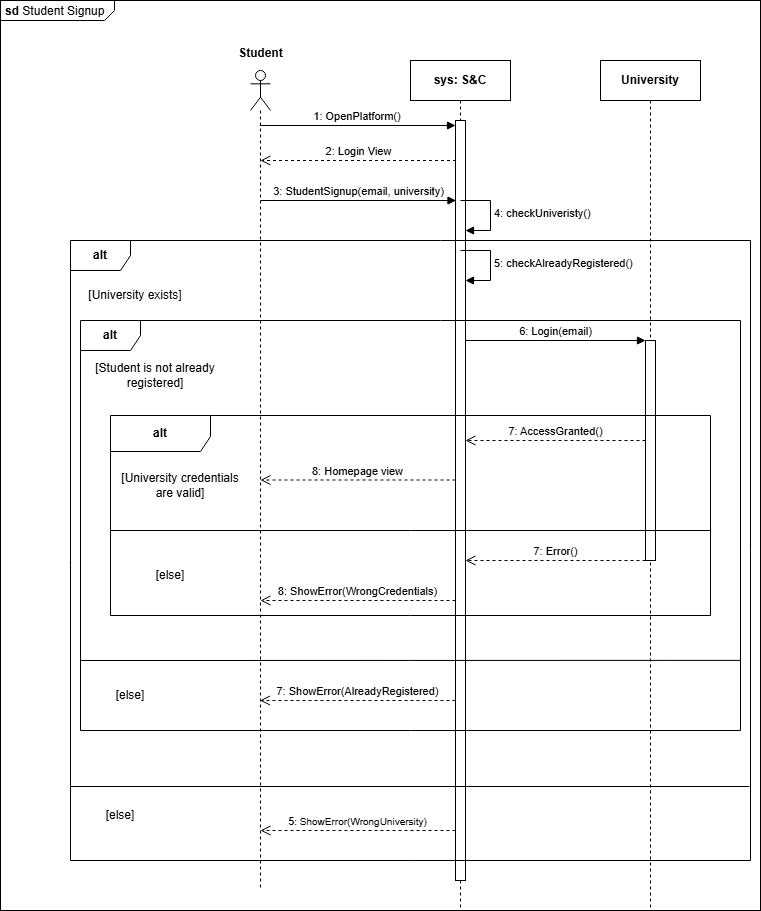
\includegraphics[width=15cm]{Images/UC_diagram/RASD-UC1.drawio.png}
    \caption{Students Signup}
\end{figure}

\begin{figure}[H]
\textbf{[UC\nextUCDiagr] Student Log in}\newline\newline
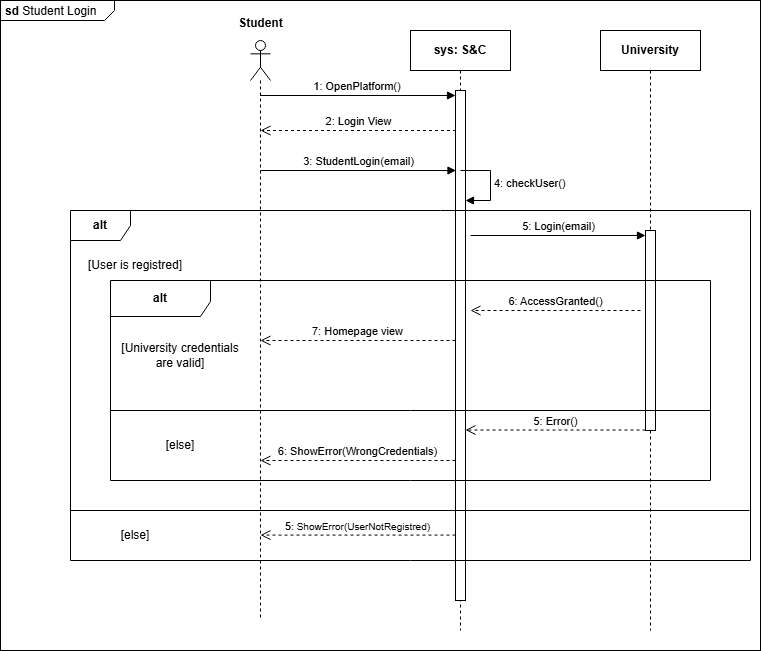
\includegraphics[width=15cm]{Images/UC_diagram/RASD-UC2.drawio.png}
    \caption{Student Log in}
\end{figure}

\begin{figure}[H]
\textbf{[UC\nextUCDiagr] Company Sign up}\newline\newline
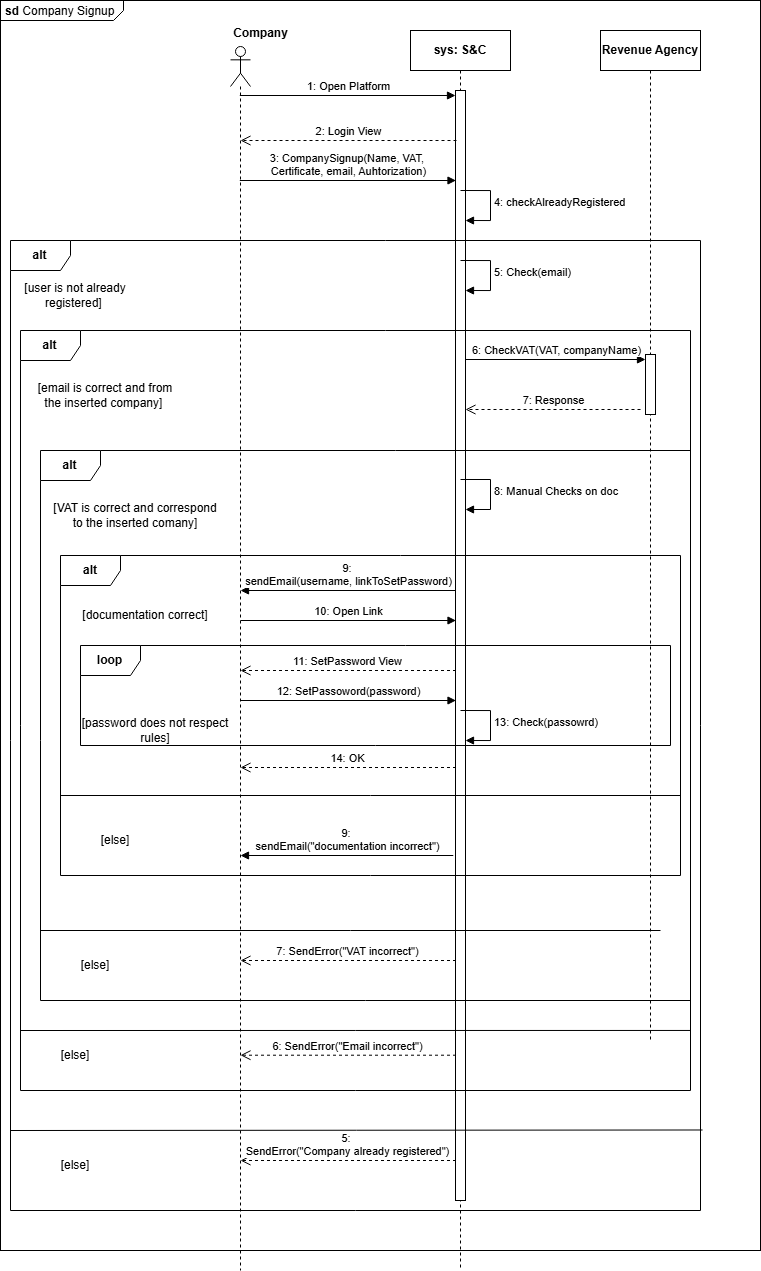
\includegraphics[width=15cm]{Images/UC_diagram/RASD-UC3.drawio (1).png}
    \caption{Company Sign up}
\end{figure}

\begin{figure}[H]
\textbf{[UC\nextUCDiagr] Company Log in}\newline\newline
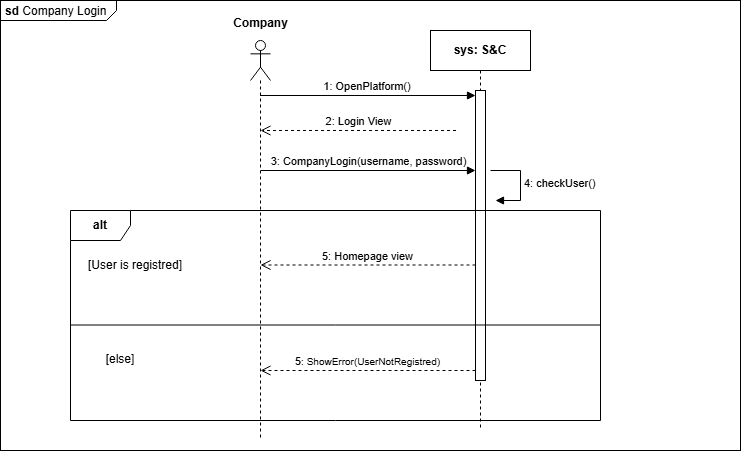
\includegraphics[width=15cm]{Images/UC_diagram/RASD-UC4.drawio.png}
    \caption{Company Log in}
\end{figure}

\begin{figure}[H]
\textbf{[UC\nextUCDiagr] Update Student's CV}\newline\newline
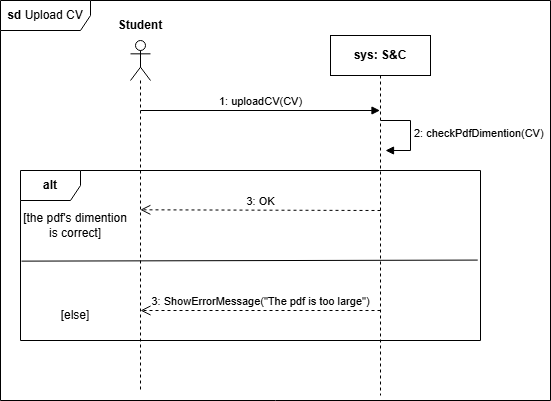
\includegraphics[width=15cm]{Images/UC_diagram/RASD-UC5.drawio.png}
    \caption{Update Student's CV}
\end{figure}

\begin{figure}[H]
\textbf{[UC\nextUCDiagr] Insert Student’s experiences, skills and/or attitudes}\newline\newline
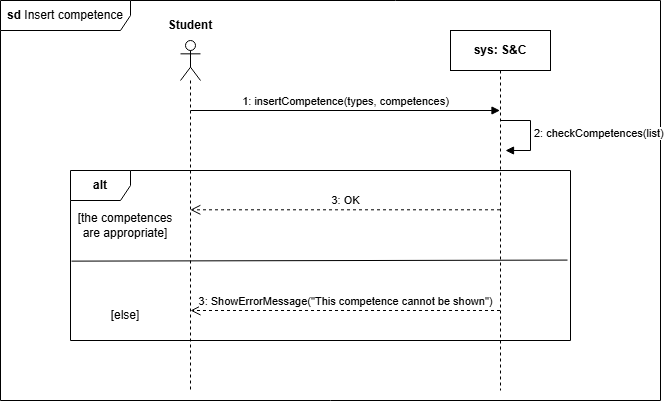
\includegraphics[width=15cm]{Images/UC_diagram/RASD-UC6.drawio.png}
    \caption{Insert Student’s experiences, skills and/or attitudes}
\end{figure}

\begin{figure}[H]
\textbf{[UC\nextUCDiagr] Edit or delete Student’s experiences, skills and/or attitudes}\newline\newline
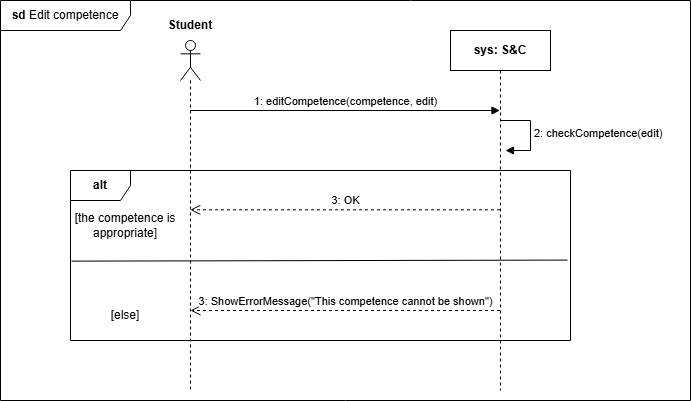
\includegraphics[width=15cm]{Images/UC_diagram/RASD-UC7.drawio.png}
    \caption{Edit or delete Student’s experiences, skills and/or attitudes}
\end{figure}

\begin{figure}[H]
\textbf{[UC\nextUCDiagr] Create internship advertising}\newline\newline
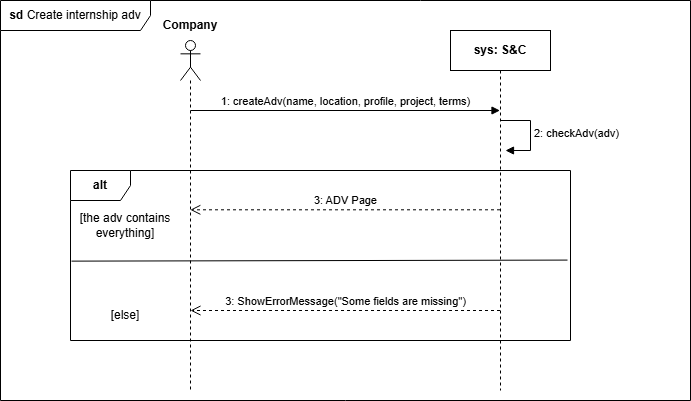
\includegraphics[width=15cm]{Images/UC_diagram/RASD-UC8.drawio.png}
    \caption{Create internship advertising}
\end{figure}

\begin{figure}[H]
\textbf{[UC\nextUCDiagr.1] Edit internship advertising}\newline\newline
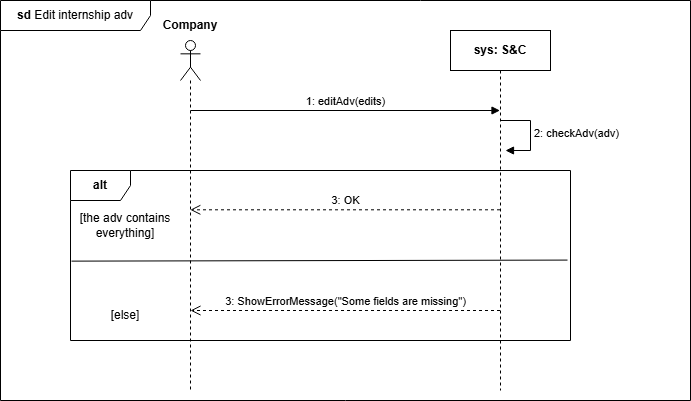
\includegraphics[width=15cm]{Images/UC_diagram/RASD-UC9.drawio.png}
    \caption{Remove internship advertising}
\end{figure}

\begin{figure}[H]
\textbf{[UC9.2] Remove internship advertising}\newline\newline
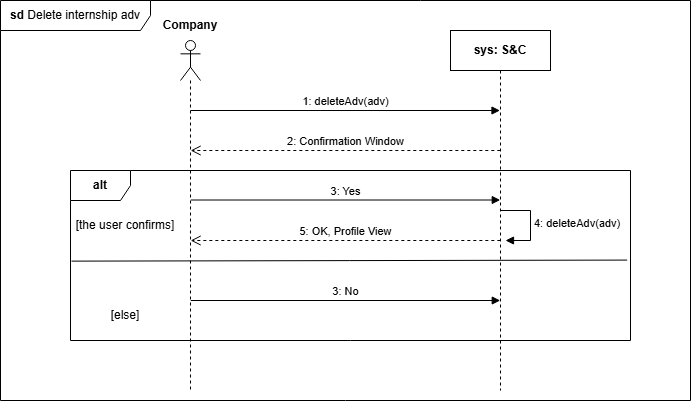
\includegraphics[width=15cm]{Images/UC_diagram/RASD-UC10.drawio.png}
    \caption{Proactive internship research}
\end{figure}

\begin{figure}[H]
\textbf{[UC\nextUCDiagr] Proactive internship research}\newline\newline
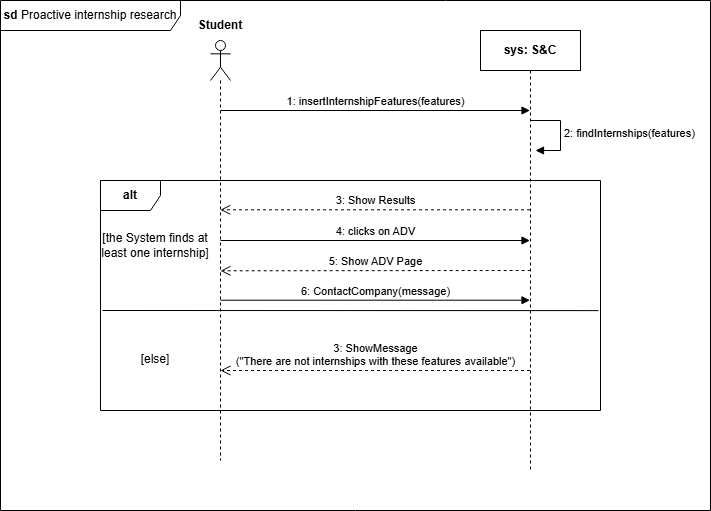
\includegraphics[width=15cm]{Images/UC_diagram/RASD-UC11.drawio.png}
    \caption{Proactive internship research}
\end{figure}

\begin{figure}[H]
\textbf{[UC\nextUCDiagr] Proactive candidates research}\newline\newline
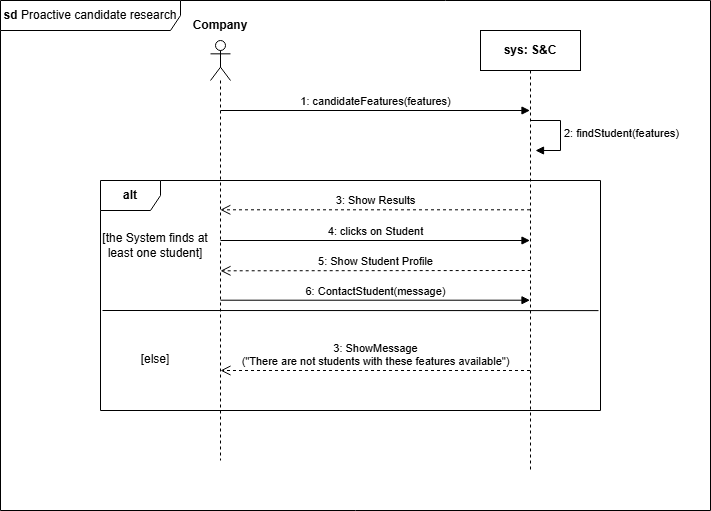
\includegraphics[width=15cm]{Images/UC_diagram/RASD-UC12.drawio.png}
    \caption{Proactive candidates research}
\end{figure}

\begin{figure}[H]
\textbf{[UC\nextUCDiagr-\nextUCDiagr-\nextUCDiagr-\nextUCDiagr] Consult Recommendations}\newline\newline
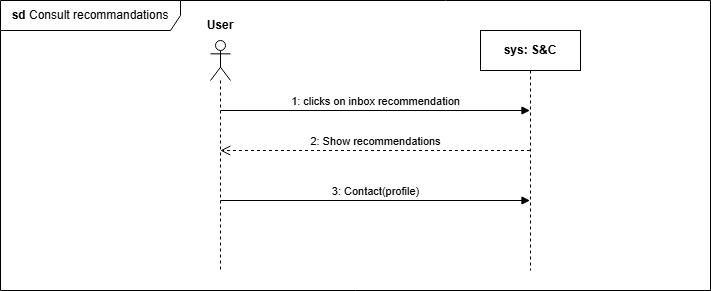
\includegraphics[width=15cm]{Images/UC_diagram/RASD-UC13.drawio.png}
    \caption{Consult Recommendations}
\end{figure}

\begin{figure}[H]
\textbf{[UC\nextUCDiagr.1] Accept internship request (Student)}\newline\newline
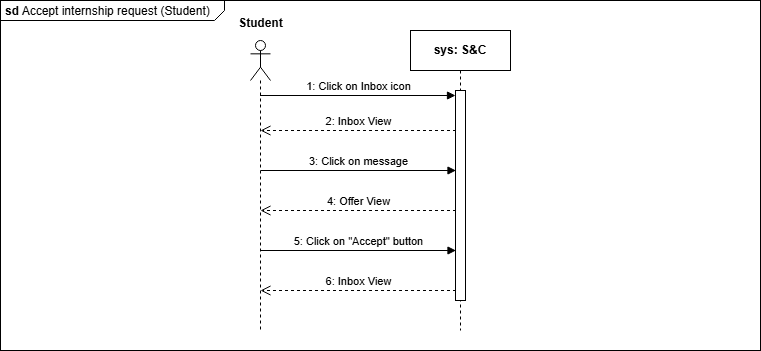
\includegraphics[width=15cm]{Images/UC_diagram/RASD-UC14.drawio.png}
    \caption{Accept internship request (Company)}
\end{figure}

\begin{figure}[H]
\textbf{[UC16.2] Reject internship request (Student)}\newline\newline
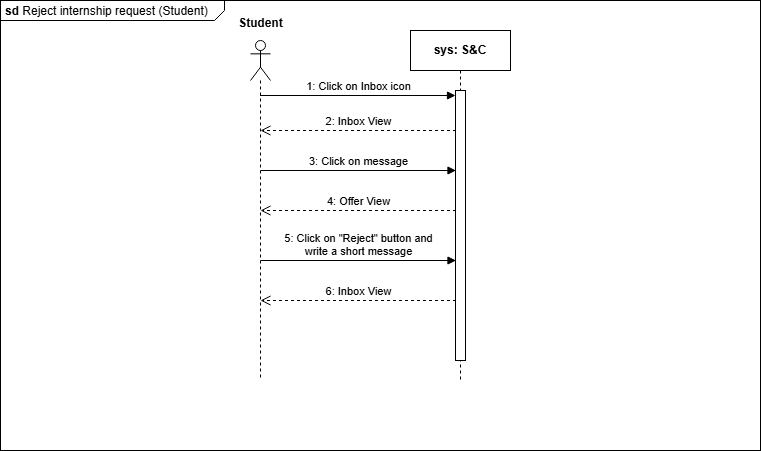
\includegraphics[width=15cm]{Images/UC_diagram/RASD-UC16.drawio.png}
    \caption{Accept internship request (Company)}
\end{figure}

\begin{figure}[H]
\textbf{[UC\nextUCDiagr.1] Accept internship request (Company)}\newline\newline
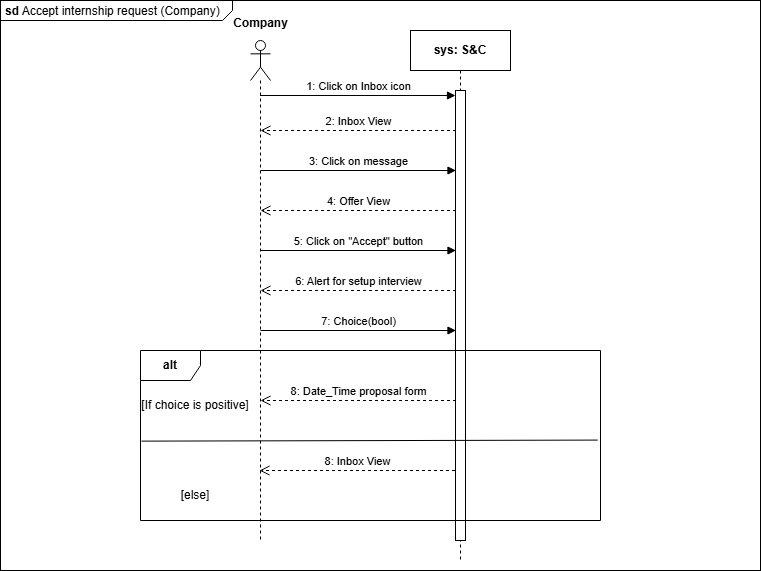
\includegraphics[width=15cm]{Images/UC_diagram/RASD-UC15.drawio.png}
    \caption{Accept internship request (Company)}
\end{figure}

\begin{figure}[H]
\textbf{[UC17.2] Reject internship request (Company)}\newline\newline
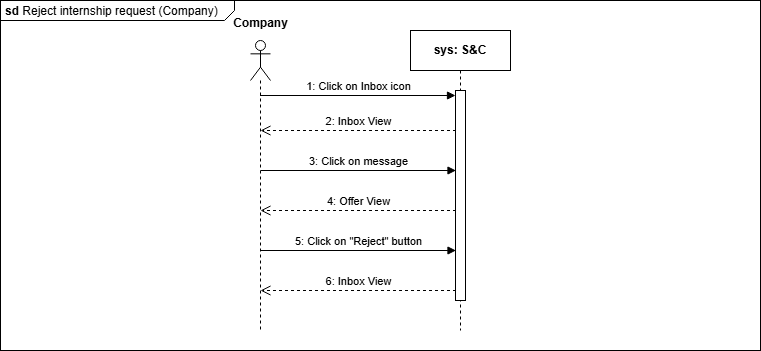
\includegraphics[width=15cm]{Images/UC_diagram/RASD-UC17.drawio.png}
    \caption{Reject internship request (Company)}
\end{figure}

\begin{figure}[H]
\textbf{[UC\nextUCDiagr] Check request outcome (Student)}\newline\newline
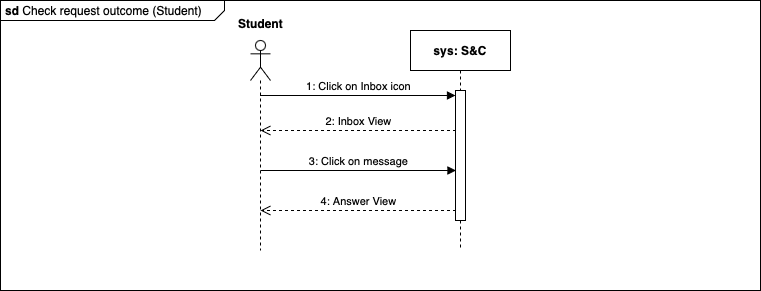
\includegraphics[width=15cm]{Images/UC_diagram/RASD-UC_CheckRequestOutcome(S).png}
    \caption{Check request outcome (Student)}
\end{figure}

\begin{figure}[H]
\textbf{[UC\nextUCDiagr] Check request outcome (Company)}\newline\newline
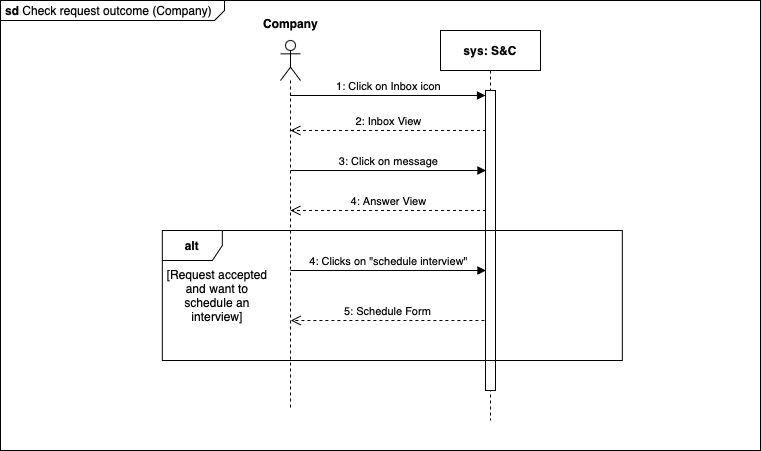
\includegraphics[width=15cm]{Images/UC_diagram/RASD-UC_CheckRequestOutcome(C).png}
    \caption{Check request outcome (Company)}
\end{figure}

\begin{figure}[H]
\textbf{[UC\nextUCDiagr.1] Propose a date for an interview}\newline\newline
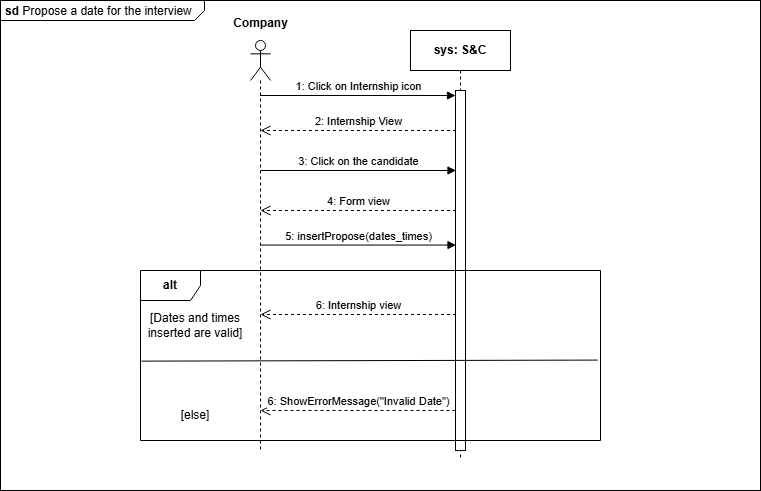
\includegraphics[width=15cm]{Images/UC_diagram/RASD-UC18.drawio.png}
    \caption{Propose a date for an interview}
\end{figure}

\begin{figure}[H]
\textbf{[UC20.2] Accepting a date for an interview}\newline\newline
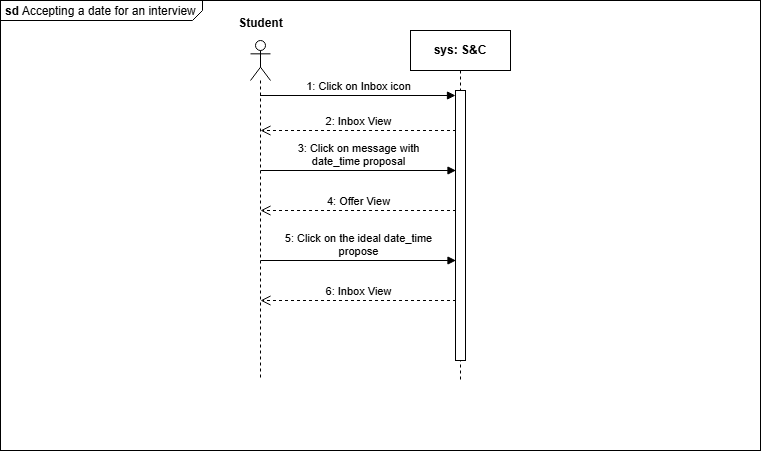
\includegraphics[width=15cm]{Images/UC_diagram/RASD-UC19.drawio.png}
    \caption{Accepting a date for an interview}
\end{figure}

\begin{figure}[H]
\textbf{[UC20.3] Reject a date for an interview}\newline\newline
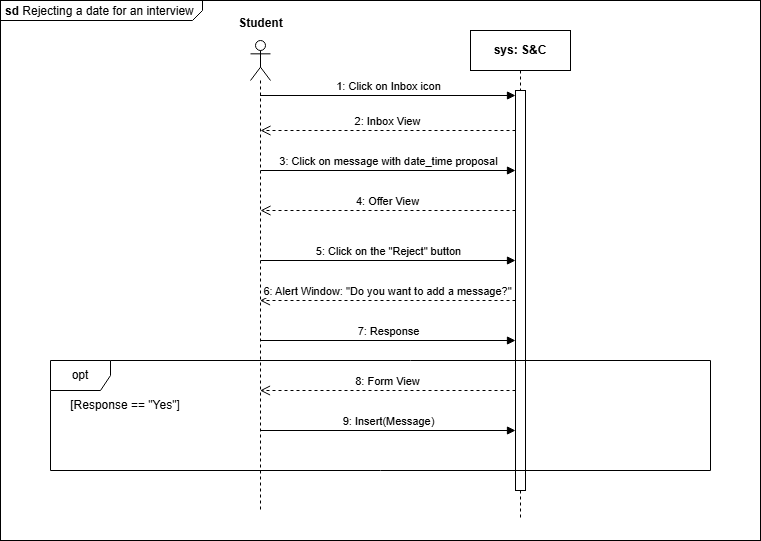
\includegraphics[width=15cm]{Images/UC_diagram/RASD-UC20.drawio.png}
    \caption{Reject a date for an interview}
\end{figure}

\begin{figure}[H]
\textbf{[UC\nextUCDiagr] Creating form for interview}\newline\newline
    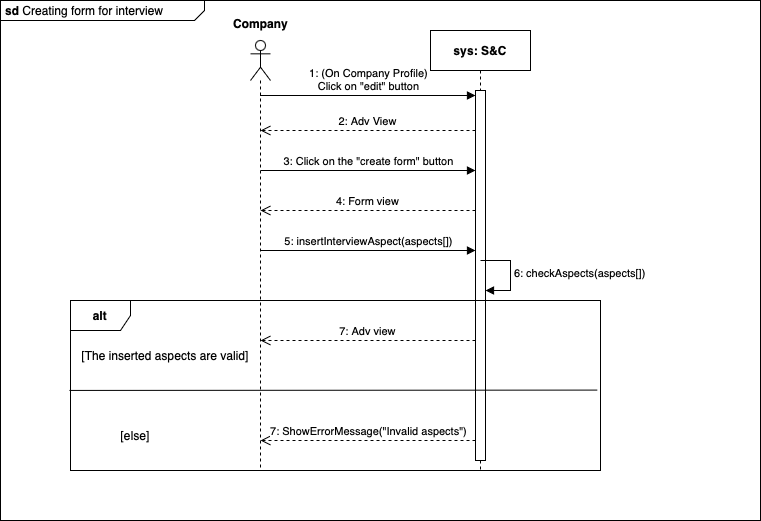
\includegraphics[width=15cm]{Images/UC_diagram/RASD-UC21(1).drawio.png}
    \caption{Creating form for interview}
\end{figure}

\begin{figure}[H]
\textbf{[UC\nextUCDiagr.1] Deleting form for interview}\newline\newline
    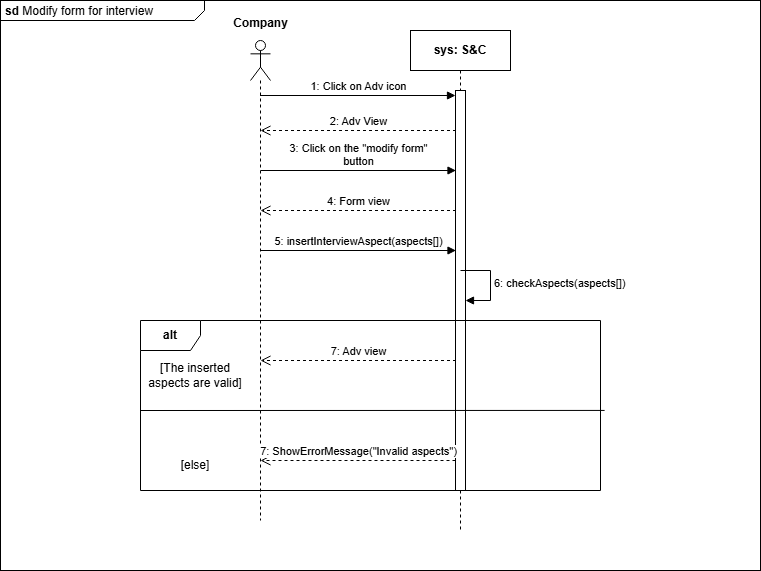
\includegraphics[width=15cm]{Images/UC_diagram/RASD-UC22.drawio.png}
    \caption{Deleting form for interview}
\end{figure}

\begin{figure}[H]
\textbf{[UC22.2 Modify form for interview}\newline\newline
    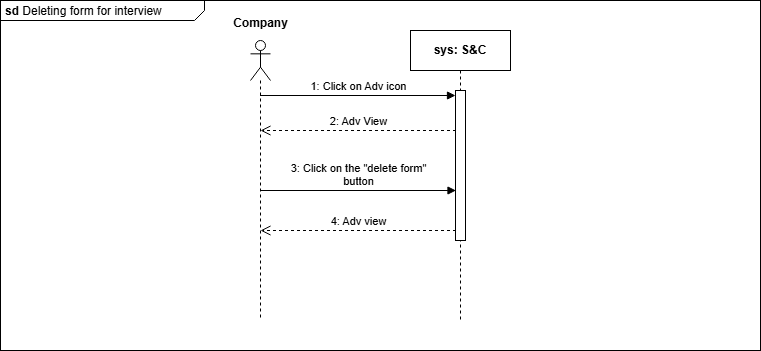
\includegraphics[width=15cm]{Images/UC_diagram/RASD-UC23.drawio.png}
    \caption{Modify form for interview}
\end{figure}

\begin{figure}[H]
\textbf{[UC\nextUCDiagr] Fill the form during interview}\newline\newline
    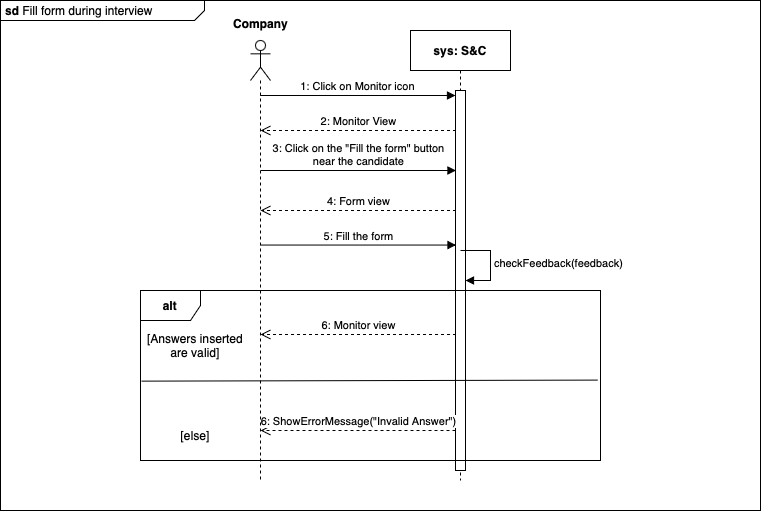
\includegraphics[width=15cm]{Images/UC_diagram/RASD-UC_FillInterviewForm.png}
    \caption{Fill the form during interview}
\end{figure}

\begin{figure}[H]
\textbf{[UC\nextUCDiagr] Feedback (Student)}\newline\newline
    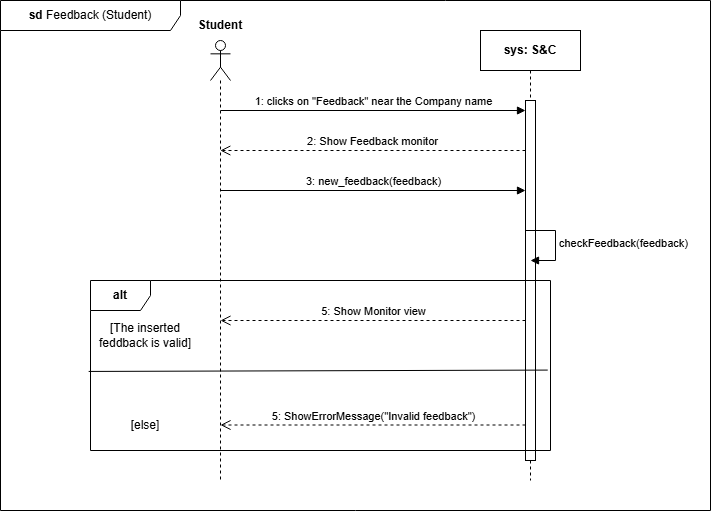
\includegraphics[width=15cm]{Images/UC_diagram/RASD-UC26.drawio.png}
    \caption{Feedback (Student)}
\end{figure}

\begin{figure}[H]
\textbf{[UC\nextUCDiagr] Feedback (Company)}\newline\newline
    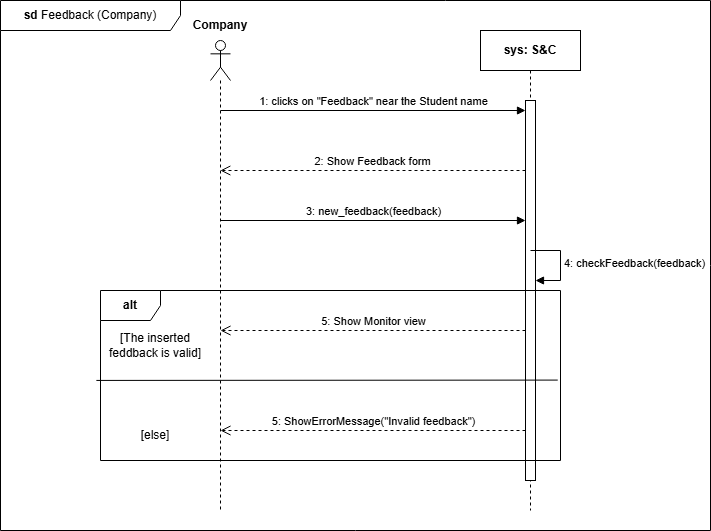
\includegraphics[width=15cm]{Images/UC_diagram/RASD-UC25.drawio.png}
    \caption{Feedback (Company)}
\end{figure}

\begin{figure}[H]
\textbf{[UC\nextUCDiagr-\nextUCDiagr-\nextUCDiagr] Monitoring}\newline\newline
    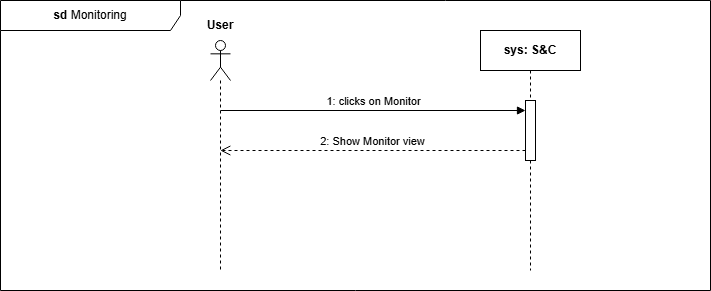
\includegraphics[width=15cm]{Images/UC_diagram/RASD-UC24.drawio.png}
    \caption{Monitoring}
\end{figure}
\subsection{Requirement Mapping}
\subsubsection{Goal-Domain Assumption-Requirement}
\begin{table}[H]
    \centering
    \begin{tabular}{|p{15cm}|}
    \hline
    {\textbf{[G1]} University students can find companies aligned with their interests, apply for internships, complete interviews, and track every stage of the process, from application to the successful completion of the internship.} \\ \hline
    \begin{itemize}
        \item[\text{[D1]}] Companies offers real internship positions.
        \item[\text{[D2]}] Students search for internship related to their course.
        \item[\text{[D3]}] Students write their CV according to their real experiences, skills and attitudes.
        \item[\text{[D4]}] The experiences, skills, and attitudes shown in the students' profiles are consistent with those in their respective CVs.
        \item[\text{[D5]}] Companies are honest in listing the projects and the terms offered.
        \item[\text{[D6]}] Students and companies are honest when giving feedback.
        \item[\text{[D7]}] Students and companies have access to a working Internet connection.
        \item[\text{[D8]}] Employees of the S\&C platform that checks the validity of a Company are capable and honest.
    \end{itemize}
    \\\hline 
    \begin{itemize}
        \item[\text{[R1]}] S\&C allows Students to sign up to the platform through their university credentials using SSO access.
        \item[\text{[R2]}] S\&C allows Student to login via their university credentials.
        \item[\text{[R5]}] S\&C allows Students to upload the PDF of their CV (both for the first time and other times if there have been some changes).
        \item[\text{[R6]}] S\&C allows Students to insert new experiences, skills, and attitudes on their profile.
        \item[\text{[R7]}] S\&C allows Students to edit or delete experiences, skills, and attitudes present on their profile.
        \item[\text{[R10]}] S\&C allows Students to use a research bar to find appropriate internship positions by inserting specific requirements about the project and/or the terms offered.
        \item [\text{[R12]}] S\&C informs students when an internship that might interest them becomes available.
        \item [\text{[R14]}] S\&C allows Students to contact a Company they are interested in.
        \item [\text{[R16]}] S\&C informs a Student when a Company shows interest in their profile by sending the Student the Company's offer. The Student can accept or decline the offer.
        \item [\text{[R18]}] S\&C communicates to Students or Companies if their requests are successful.
        \item [\text{[R19]}] S\&C allows Companies to setup an interview with the candidates.
        \item [\text{[R24]}] S\&C allows Companies to give feedback during the internship about a single Student.
        \item [\text{[R25]}] S\&C offers Students the possibility to monitor their matchmaking process with a Company (state of the matchmaking, scheduled interview, interview results).
        \item [\text{[R27]}] S\&C offers Students and Companies the possibility to monitor the state of the internship.
    \end{itemize}
    
    \\ \hline
    \end{tabular}
\end{table}

\begin{table}[H]
    \centering
    \begin{tabular}{|p{15cm}|}
    \hline
    {\textbf{[G2]} Companies can advertise their internship opportunities to find suitable students for the position, contact them, conduct interviews, hire the best candidates, and keep track of the entire process.} 
    \\\hline \begin{itemize}
        \item[\text{[D3]}] Students write their CVs according to their real experiences, skills and attitudes.
        \item[\text{[D4]}] The experiences, skills, and attitudes shown in the students' profiles are consistent with those in their respective CVs. 
        \item[\text{[D6]}] Students and companies are honest when giving feedback.
        \item[\text{[D7]}] Students and companies have access to a working Internet connection.
    \end{itemize}\\ \hline
    \begin{itemize}
         \item[\text{[R3]}] S\&C allows Companies to sign up to the platform by asking the representative of the company to insert their company email, the VAT number of the company, a Certificate of registration at the Chamber of Commerce, and a letter of authorisation or official assignment signed by a CEO or a HR referent. They have to choose a password.
        \item[\text{[R4]}] S\&C allows Companies to login to the platform via password and username (created by the system).
        \item[\text{[R8]}] S\&C allows Companies to create an advertisement regarding an internship position they are offering, explaining the project of the internship and the terms offered.
    
        \item[\text{[R9]}] S\&C allows Companies to modify and remove an advertisement posted on their page.
        \item[\text{[R11]}] S\&C allows Companies to use a research bar to find appropriate candidates for their internship positions by inserting specific experiences, skills and/or attitudes the candidates should have.
        \item [\text{[R13]}] S\&C informs companies about the availability of a student whose CV corresponds to their needs.
        \item [\text{[R14]}] S\&C allows Students to contact a Company they are interested in.
        \item [\text{[R15]}] S\&C allows Companies to contact Students they are interested in.
        \item [\text{[R16]}] S\&C informs a Student when a Company shows interest in their profile by sending the Student the Company's offer. The Student can accept or decline the offer.
    
        \item [\text{[R17]}] S\&C informs a Company when a Student shows interest in its offer by sending to the Company the Student's CV, the Company can accept or decline the offer.
    
        \item [\text{[R18]}] S\&C communicates to Students or Companies if their requests are successful.
    \item [\text{[R19]}] S\&C allows Companies to setup an interview with the candidates.
    
        \item [\text{[R20]}] S\&C allows Companies to write a form with all the aspects that will be considered during the interviews.
    
        \item [\text{[R21]}] S\&C allows Companies to modify or delete the interview form created.
        \item [\text{[R22]}] S\&C allows Companies fill the form during the interview.
        \item [\text{[R23]}] S\&C allows Students to give personal feedback during the selection period about the Company's selection method or during the internship period about the internship itself.
        \item [\text{[R26]}] S\&C offers Companies the possibility to monitor their matchmaking process with a Student.
    
        \item [\text{[R27]}] S\&C offers Students and Companies the possibility to monitor the state of the internship.
    \end{itemize}
     \\ \hline
    \end{tabular}
\end{table}

\subsubsection{Requirement - Use Case}
\begin{table}[H]
    \centering
    \begin{tabular}{|p{10cm}|p{5cm}|}
    \hline
         [R1] S\&C allows Students to sign up to the platform through their university credentials using SSO access. & [UC1] Students Signup \\ \hline
         [R2] S\&C allows Student to login via their university credentials.& [UC2] Students Login\\\hline
         [R3] S\&C allows Companies to sign up to the platform by asking the representative of the company to insert their company email, the VAT number of the company, a Certificate of registration at the Chamber of Commerce, and a letter of authorisation or official assignment signed by a CEO or a HR referent. They have to choose a password. &[UC3] Company Sign up \\\hline
         [R4] S\&C allows Companies to login to the platform via password and username (created by the system). & [UC4] Company Login\\\hline
         [R5] S\&C allows Students to upload the PDF of their CV (both for the first time and other times if there have been some changes).[UC5] Update student’s CV & [UC5] Update student’s CV\\\hline
         [R6] S\&C allows Students to insert new experiences, skills, and attitudes on their profile.& [UC6] Insert Student’s experiences, skills and/or attitudes\\\hline
         [R7] S\&C allows Students to edit or delete experiences, skills, and attitudes present on their profile.&[UC7] Edit or delete Student’s experiences, skills and/or attitudes \\\hline
         [R8] S\&C allows Companies to create an advertisement regarding an internship position they are offering, explaining the project of the internship and the terms offered. &[UC8] Create internship advertising \\\hline
         [R9] S\&C allows Companies to modify and remove an advertisement posted on their page.&[UC9.1] Edit internship advertising\newline[UC9.2] Remove internship advertising \\\hline
         [R10] S\&C allows Students to use a research bar to find appropriate internship positions by inserting specific requirements about the project and/or the terms offered. & [UC10] Proactive internship research \\\hline
         [R11] S\&C allows Companies to use a research bar to find appropriate candidates for their internship positions by inserting specific experiences, skills and/or attitudes the candidates should have. & [UC11] Proactive candidates research\\\hline
         [R12] S\&C informs students when an internship that might interest them becomes available. \newline [R13] S\&C informs companies about the availability of a student whose CV corresponds to their needs. \newline [R14] S\&C allows Students to contact a Company they are interested in. \newline [R15] S\&C allows Companies to contact Students they are interested in. & [UC12-13-14-15] Consult Recommendations\\\hline
     \end{tabular}
\end{table}
\begin{table}[H]
    \centering
    \begin{tabular}{|p{10cm}|p{5cm}|}
    \hline
         [R16]  S\&C informs a Student when a Company shows interest in their profile by sending the Student the Company's offer. The Student can accept or decline the offer. & [UC16.1] Accept internship request (Student) \newline [UC16.2] Reject internship request (Student)\\\hline
         [R17] S\&C informs a Company when a Student shows interest in its offer by sending to the Company the Student's CV, the Company can accept or decline the offer. & [UC17.1] Accept internship request (Company) \newline [UC17.2] Reject internship request (Company) \\\hline
         [R18] S\&C communicates to Students or Companies if their requests are successful. &[UC18.1] Check request outcome (Student)\newline [UC18.2] Check request outcome (Company)\\\hline
         [R19] S\&C allows Companies to setup an interview with the candidates. & [UC19.1] Propose a date for an interview\newline [UC19.2] Accepting a date for an interview\newline[UC19.3] Reject a date for an interview \\\hline
         [R20] S\&C allows Companies to write a form with all the aspects that will be considered during the interviews.& [UC20] Creating form for interview\\\hline
         [R21] S\&C allows Companies to modify or delete the interview form created. & [UC21.1] Deleting form for interview \newline [UC21.2] Modify form for interview\\\hline
         [R22] S\&C allows Companies fill the form during the interview. & [UC22] Fill the form for interview\\\hline
         [R23] S\&C allows Students to give personal feedback during the selection period about the Company's selection method or during the internship period about the internship itself. & [UC23] Feedback (Student)\\\hline
         [R24] S\&C allows Companies to give feedback during the internship about a single Student. & [UC24] Feedback (Company)\\\hline
         [R25] S\&C offers Students the possibility to monitor their matchmaking process with a Company (state of the matchmaking, scheduled interview, interview results).\newline [R26] S\&C offers Companies the possibility to monitor their matchmaking process with a Student.\newline S\&C offers Students and Companies the possibility to monitor the state of the internship. & [UC25-26-27] Monitoring\\\hline
    \end{tabular}
\end{table}
\section{Performance Requirements}
\subsection{Number of Users}
In Italy, in 2022, approximately 173 000 university students participated in internships. There are 40,000 Italian companies registered on LinkedIn, and about 70\% of them (equivalent to 28 000) offer internship opportunities to university students. Therefore, the total number of potential users for a website like S\&C in Italy could be around 201 000. Our platform could capture 30\% of this audience, which amounts to approximately \textbf{60 000 users}.
\subsection{Data Storage}
Here is the amount of storage needed categorised:
\begin{itemize}
    \item \textbf{Student's profile}: we consider the average case in which the student uploads the PDF of their CV (maximum 1 MB) and about 10 competences. For each competence, we have to store name (string of length 15/20 chars, i.e. 16-21 bytes), type (char: S-skill, E-experience, A- attitude, i.e. 1 byte), and small description (text of about 2 lines, i.e. 161 bytes), plus an overhead of 7-14 bytes, so, one competence takes up about 191 bytes, consequentially, 10 competences take up about 1,9 KB. We have also to consider the email and the name of the university, both around 35 bytes. So, in total, the storage of the personal information of a student takes up about 1001,97 KB, i.e. 1 MB.
    \item \textbf{Company's profile and ADVs}: for each company, we store the name (string of length 40/50 chars, i.e. 41-51 bytes), the VAT number (11 chars, i.e. 11 bytes), representative's email (35 bytes), password (SHA-256, i.e. 64 chars, i.e. 64 bytes), Certificate of registration at the Chamber of Commerce (500 KB). On average each company could have about 3 Internship Advertisements. For each ADV, we have to store: name (string of length 40/50 chars, i.e. 41-51 bytes), location (30 bytes), candidate profile (500 bytes), project description (1000 bytes), terms offered (500 bytes), interview form (it depends on the amount of fields, on average 3.4 KB). So, for an average company we need about 517 KB.
    \item \textbf{Matches and Recommendations}: both are linked to the users and ADVs involved (so we need their IDs, i.e. 4 bytes each); the matches contain also the status (recognised by a char, so 1 byte). So for a match, we need about 9 bytes, and for a recommendation about 8 bytes. 
    \item \textbf{Feedback}: it will have the IDs of the users involved (8 bytes in total), the comment (about 500 bytes), and the fields regarding the checks to be done on the user profile (about 300 bytes). In total, about 800 bytes.
\end{itemize}
\subsection{Time Response}
Each operation performed by the S\&C platform should be completed within milliseconds, except for the manual control of company registrations.
\section{Design Constraints}
\subsection{Standards Compliance}
The S\&C platform ensures compliance with GDPR (General Data Protection Regulation) for data protection, WCAG (Web Content Accessibility Guidelines) for accessibility, and OWASP (Open Web Application Security Project) to prevent security issues. It uses W3C standards (World Wide Web Consortium) for compatibility and responsive design to support all devices. It implements HTTPS for safe communication and follows ISO/IEC 27001 (Information Security Management) to protect data effectively.
\subsection{Hardware Limitation}
The only limitation for the device concerns the internet connection and a portable device which supports the app or a computer with a Web Browser.
\section{Software System Attributes}
\subsection{Reliability}
The system implements reliability with robust error handling and automatic retries for unsuccessful API calls. 
\subsection{Availability}
The platform is always accessible, maintaining a high availability targeting a 99.9\% uptime ("three nines"), this way the system will be unavailable only for 8.76 hours per year. It uses load balancing to handle high traffic efficiently.
\subsection{Security}
The system must control the User access (Company and Student), verify identity through university credentials for Students and insert VAT number and upload a certificate of the Chamber of Commerce for Companies. Some measure to protect the databases, with all the information, will be adopted, like encryption of personal data and protection against query injections.
\subsection{Maintainability}
The system requires manual intervention only for authorizing Companies Sign up. The ordinary maintenance has to be scheduled during nighttime in order to guarantee the maximum uptime.
\subsection{Portability}
The system is a web application so it must be viewable on different web browsers and devices with different screen proportions.


\pagebreak
\chapter{Formal Analysis Using Alloy}

\section{Alloy model}
\begin{lstlisting}
open util/boolean
sig System {
	has : set User,
	creates : set Recommendation,
	accumulates : set Match
}

abstract sig User {
	sends : set InternshipRequest,
	receives : set InternshipRequest,
	gets : set Recommendation,
	isProposed : set Recommendation
}{
	one s : System | this in s.has
}

sig Student extends User {
	has : set Competence,
	joins : set Match
}

sig Competence {}{
	one s : Student | this in s.has
}

sig Company extends User {
	creates : set InternshipAdv
}{}

sig InternshipAdv {
	includes : lone InterviewForm,
	collects : set InternshipRequest,
	isInserted : set Recommendation,
	partecipates : set Match
}{
	one c : Company | this in c.creates
}

sig InternshipRequest {
	isAccepted : Bool
}{
	one adv : InternshipAdv | this in adv.collects
	one sender : User | this in sender.sends
	one receiver : User | this in receiver.receives
}

sig Recommendation {}{
	one receiver :  User | this in receiver.gets
	one proposed : User | this in proposed.isProposed
	one adv : InternshipAdv | this in adv.isInserted
	one s : System | this in s.creates
}

sig Match {
	executes : one Interview,
	var status : one MatchmakingStatus,
	gathers : set Feedback
}{
	one s : System | this in s.accumulates
	one adv : InternshipAdv | this in adv.partecipates
	one stud : Student | this in stud.joins
}

enum MatchmakingStatus{
	INTERVIEW_SET, INTERVIEW_COMPLETED, INTERNSHIP_ACCEPTED, INTERNSHIP_DECLINED, INTERNSHIP_FIRST_HALF, INTERNSHIP_COMPLETED
}

sig Interview {}{
	one m : Match | this in m.executes
}

sig InterviewForm {}{
	one adv : InternshipAdv | this in adv.includes
}

sig Feedback {
	direction : FeedbackDirection,
	status : one MatchmakingStatus
}{
	one m : Match | this in m.gathers
}

enum FeedbackDirection{
	S2C, C2S
}


//----------------------------FACTS----------------------------
fact UniqueSystem {
	#System = 1
}
//InternshipRequest
//check that InternshipRequest are c->s or s->c
fact NOInternshipRequest_C2C {
	no req : InternshipRequest, c1 : Company, c2 : Company |
		(req in c1.sends and req in c2.receives)
}
fact NOInternshipRequest_S2S {
	no req : InternshipRequest,  s1 : Student, s2 : Student |
		(req in s1.sends and req in s2.receives)
}

//The adv inside the internship request is created by the company that sends (or receives) that internship request 
fact InternshipRequest_C_owns_Adv {
	all req : InternshipRequest, c : Company, adv : InternshipAdv |
		(req in adv.collects and (req in c.sends or req in c.receives)) implies (adv in c.creates)
}

//There are not multiple internship request with the same fields
fact UniqueInternshipRequest{
	all u_sender : User, u_reciver : User, adv : InternshipAdv | no disj req1, req2 : InternshipRequest |
		(req1 in u_sender.sends and req1 in u_reciver.receives and req1 in adv.collects and 
		req2 in u_sender.sends and req2 in u_reciver.receives and req2 in adv.collects)
}
//There are not bidirectional request (a student S1 to a company C1 and C1 to S1)
fact NoBidirectionalInternshipRequest{
	all req1 : InternshipRequest, req2 : InternshipRequest , u_sender : User, u_reciver : User, adv : InternshipAdv |
		(req1 in u_sender.sends and req1 in u_reciver.receives and req1 in adv.collects) 
		implies not
		(req2 in u_sender.receives and req2 in u_reciver.sends and req2 in adv.collects)
}

//Recommendation
//Recommendation can not be company2company or student2student
fact NORecommendation_C2C {
	no reco : Recommendation, c1 : Company, c2 : Company |
		(reco in c1.isProposed and reco in c2.gets)
}
fact NORecommendation_S2S {
	no reco : Recommendation,  s1 : Student, s2 : Student |
		(reco in s1.isProposed and reco in s2.gets)
}

//The adv inside the recommendation is created by the company that gets (or is proposed in) that recommendation 
fact Recommendation_C_owns_Adv {
	all reco : Recommendation, c : Company, adv : InternshipAdv |
		(reco in adv.isInserted and (reco in c.isProposed or reco in c.gets)) implies (adv in c.creates)
}

//There are not multiple recommendation with the same fields
fact UniqueRecommendation{
	all u_proposed : User, u_getter : User, adv : InternshipAdv | no disj reco1, reco2 : Recommendation |
		(reco1 in u_proposed.isProposed and reco1 in u_getter.gets and reco1 in adv.isInserted and 
		reco2 in u_proposed.isProposed and reco2 in u_getter.gets and reco2 in adv.isInserted)
}

//Match
//There are not multiple match with the same fields
fact CreateUniqueMatchPerRequest {
    	all s : Student, adv : InternshipAdv, req : InternshipRequest | 
		((req in s.sends or req in s.receives) and req in adv.collects and req.isAccepted in True)
       		implies one m : Match |
            	(m in s.joins and m in adv.partecipates)
}
fact CreateUniqueMatchPerRequest2 {
    	all m : Match, s : Student, adv : InternshipAdv | 
		(m in s.joins and m in adv.partecipates)
		implies one req : InternshipRequest |
		((req in s.sends or req in s.receives) and req in adv.collects and req.isAccepted in True)
}
fact UniqueMatch{
	all s : Student, adv : InternshipAdv | no disj m1, m2 : Match |
		(m1 in s.joins and  m1 in adv.partecipates and 
		m2 in s.joins and m2 in adv.partecipates)
}

//State Machine for successful match (will lead to a internship)
pred MatchProgress[m : Match]{
		m.status = INTERVIEW_SET   and eventually (m.status = INTERVIEW_COMPLETED)
			and always(m.status = INTERVIEW_COMPLETED implies eventually m.status = INTERNSHIP_ACCEPTED
					and always (m.status = INTERNSHIP_ACCEPTED implies eventually (m.status = INTERNSHIP_FIRST_HALF)
						and always (m.status = INTERNSHIP_FIRST_HALF implies eventually m.status = INTERNSHIP_COMPLETED
							and always (m.status = INTERNSHIP_COMPLETED implies always m.status = INTERNSHIP_COMPLETED)
						)
					)
				)
		
}

//State Machine for unsuccessful match (will not lead to a internship)
pred MatchProgressDeclined[m : Match]{
		m.status = INTERVIEW_SET   and eventually (m.status = INTERVIEW_COMPLETED)
			and always(m.status = INTERVIEW_COMPLETED implies eventually m.status = INTERNSHIP_DECLINED
					and always (m.status = INTERNSHIP_DECLINED implies always m.status = INTERNSHIP_DECLINED))
}

//InterviewForm
//An interview cannot occour without an InterviewForm
fact NoInterviewWithoutForm {
	all i : Interview, m : Match, adv : InternshipAdv |
		(i in m.executes and m in adv.partecipates) implies one form : InterviewForm | form in adv.includes 
}

//Feedback
//There are not multiple feedback with the same fields
fact UniqueFeedback {
	all m: Match | no disj f1, f2 : Feedback | (f1 in m.gathers and f2 in m.gathers and f1.status = f2.status and f1.direction = f2.direction)
}
//Feedback cannot be write in INTERVIEW_SET, INTERNSHIP_ACCEPTED or INTERNSHIP_DECLINED status
fact ImpossibleFeedbackStatus {
	no f : Feedback | f.status = INTERVIEW_SET or f.status = INTERNSHIP_ACCEPTED or  f.status = INTERNSHIP_DECLINED
}

//Feedback cannot be wrote in status that has not be reached yet 
fact NoFeedbackFutureState {
	all m : Match |
		((m.status = INTERNSHIP_COMPLETED and #m.gathers > 0 ) implies all f : m.gathers |  (f.status = INTERVIEW_COMPLETED or f.status = INTERNSHIP_FIRST_HALF or f.status = INTERNSHIP_COMPLETED))
		and
		((m.status = INTERNSHIP_FIRST_HALF and #m.gathers > 0 ) implies all f : m.gathers |  (f.status = INTERVIEW_COMPLETED or f.status = INTERNSHIP_FIRST_HALF))
		and
		(((	m.status = INTERVIEW_COMPLETED 
			or m.status = INTERNSHIP_ACCEPTED 
			or m.status = INTERNSHIP_DECLINED ) and #m.gathers > 0 ) implies all f : Feedback | f in m.gathers and f.status = INTERVIEW_COMPLETED)
		and
		(m.status = INTERVIEW_SET) implies m.gathers = none
}
fact NoFeedbackFutureState2 {
	all f : Feedback |
		((f.status = INTERVIEW_COMPLETED) implies one m : Match | f in m.gathers and (m.status = INTERVIEW_COMPLETED or m.status = INTERNSHIP_ACCEPTED or m.status = INTERNSHIP_DECLINED or m.status = INTERNSHIP_FIRST_HALF or m.status = INTERNSHIP_COMPLETED))
		and
		((f.status =  INTERNSHIP_FIRST_HALF) implies one m : Match | f in m.gathers and (m.status = INTERNSHIP_FIRST_HALF or m.status = INTERNSHIP_COMPLETED))
		and
		((f.status = INTERNSHIP_COMPLETED) implies one m : Match | f in m.gathers and  m.status = INTERNSHIP_COMPLETED)
}
//----------------------------ASSERTION----------------------------
//Check that the maximum number of feedback linked to a match cannot be over 6 (3 possible states and 2 direction for each)
assert moreThan6FeedbackPerMatch {
	all m : Match | #m.gathers < 7}


\end{lstlisting}
\clearpage
\subsection{Example}

\subsubsection{Base World}
\begin{lstlisting}
pred baseWorld {
	//Student
	#Student = 1
	#Competence = 0
	//Company
	#Company = 1
	#InternshipAdv = 1
	//S&C
	#Recommendation = 0
	#InternshipRequest = 0
	#Match = 0
	#Feedback = 0
}
run baseWorld for 6
\end{lstlisting}

\begin{figure}[h]
    \centering
    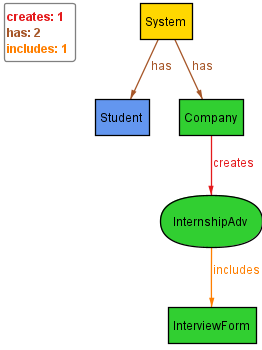
\includegraphics[width=0.5\textwidth]{Images/AlloyModel_images/baseWorld.png}
    \caption{baseWorld}
    \label{fig:figure2}
\end{figure}
Example of the simplest (initial) structure with only one Student and one Company which created an InternshipAdv and an InterviewForm for that ADV.

%------------------------------------------------
\clearpage

\subsubsection{Base World with Recommendation}
\begin{lstlisting}
pred baseWorldWithRecommendation {
	//Student
	#Student = 1
	#Competence = 0
	//Company
	#Company = 1
	#InternshipAdv = 1
	//S&C
	#Recommendation = 1
	#InternshipRequest = 0
	#Match = 0
	#Feedback = 0
}
run baseWorldWithRecommendation for 6
\end{lstlisting}

\begin{figure}[h]
    \centering
    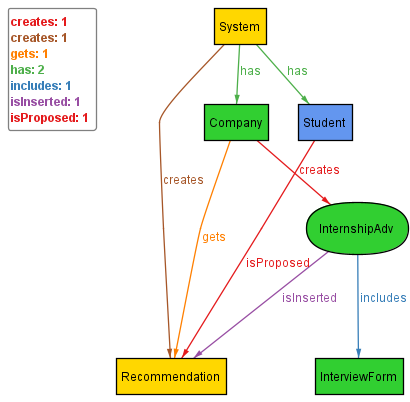
\includegraphics[width=0.75\textwidth]{Images/AlloyModel_images/baseWorldWithRecommendation.png}
    \caption{baseWorldWithRecommendation}
    \label{fig:figure2}
\end{figure}
Example of a structure with only one Student and one Company which created an InternshipAdv and an InterviewForm for that adv. Then the System creates a Recommendation for the Company where a Student is proposed.

%------------------------------------------------
\clearpage

\subsubsection{Base World with Match}
\begin{lstlisting}

pred baseWorldWithMatch {
	//Student
	#Student = 1
	#Competence = 0
	//Company
	#Company = 1
	#InternshipAdv = 1
	//S&C
	#Recommendation = 0
	#Match = 1
	#Feedback = 0
}
run baseWorldWithMatch for 6
\end{lstlisting}

\begin{figure}[h]
    \centering
    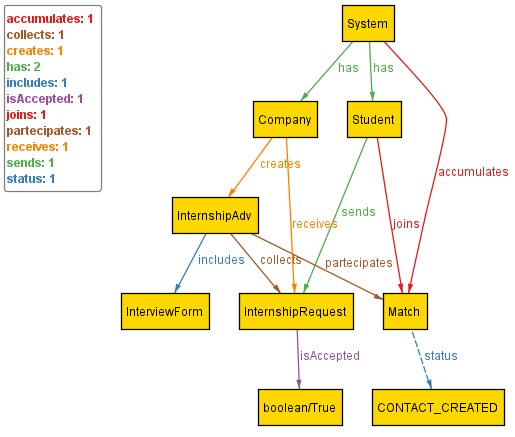
\includegraphics[width=0.8\textwidth]{Images/AlloyModel_images/baseWorldWithMatch.png}
    \caption{baseWorldWithMatch}
    \label{fig:figure2}
\end{figure}
Example of a structure with only one Student and one Company which created an InternshipAdv and an InterviewForm for that adv. The Student sends a InternshipRequest to the Company for the InternshipAdv, the request was accepted (boolean True) so a Match was created and the interview was execute, the status of the Match is INTERNSHIP\_DECLINED.

%------------------------------------------------
\clearpage

\subsubsection{Base World with Match Request Denied}
\begin{lstlisting}
pred baseWorldWithMatchRequestDenied {
	//Student
	#Student = 2
	#Competence = 0
	//Company
	#Company = 1
	#InternshipAdv = 1
	//S&C
	#InternshipRequest = 2
	#Recommendation = 0
	#Match = 1
	#Feedback = 0
}
run baseWorldWithMatchRequestDenied for 6
\end{lstlisting}

\begin{figure}[h]
    \centering
    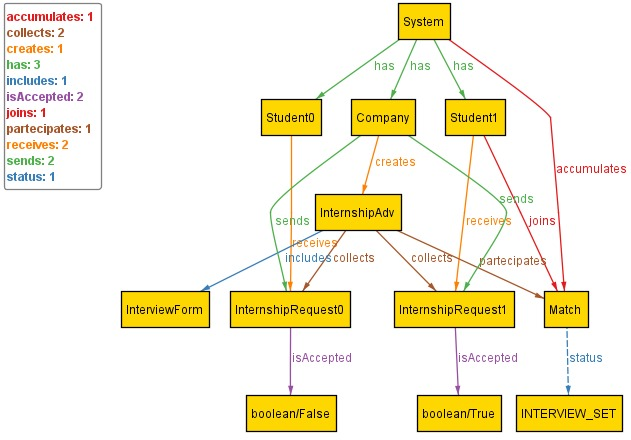
\includegraphics[width=0.9\textwidth]{Images/AlloyModel_images/baseWorldWithMatchRequestDenied.png}
    \caption{baseWorldWithMatchRequestDenied}
    \label{fig:figure2}
\end{figure}
Example of a structure with two Student and one Company which created an InternshipAdv and an InterviewForm for that adv. The Students send an InternshipRequest to the Company for the InternshipAdv, one request was declined (Student0) and one accepted (Student1) so a Match was created.

%------------------------------------------------
\clearpage

\subsubsection{Base World with Feedback}
\begin{lstlisting}
pred baseWorldWithFeedbacks {
	//Student
	#Student = 1
	#Competence = 0
	//Company
	#Company = 1
	#InternshipAdv = 1
	//S&C
	#Recommendation = 0
	#Match = 1
	#Feedback = 4
}
run baseWorldWithFeedbacks for 6
\end{lstlisting}

\begin{figure}[h]
    \centering
    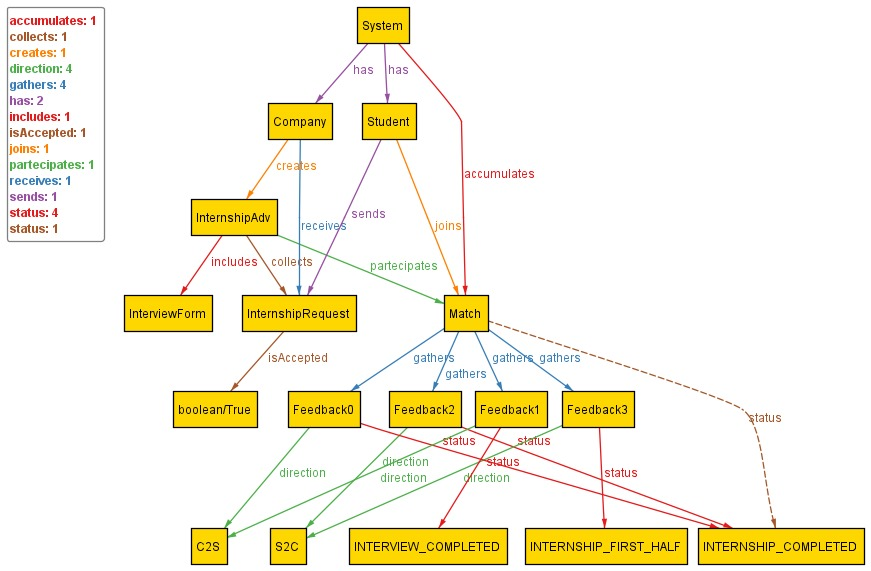
\includegraphics[width=1\textwidth]{Images/AlloyModel_images/WorldWithFeedbacks.png}
    \caption{baseWorldWithFeedbacks}
    \label{fig:figure2}
\end{figure}
Example of a structure with only one Student and one Company which created an InternshipAdv and an InterviewForm for that adv. The Student sends a InternshipRequest to the Company for the InternshipAdv, the request was accepted (boolean True) so a Match was created, the current Status of the Match is INTERNSHIP\_COMPLETED and four Feedbacks were writed: two for the status INTERNSHIP\_FIRST\_HALF (one from Company and one from Student) and the other two for the status INTERNSHIP\_COMPLETED (one from Company and one from Student).\newline

%------------------------------------------------
%\clearpage

\begin{lstlisting}
assert moreThan6FeedbackPerMatch {
	all m : Match | #m.gathers < 7
}
check moreThan6FeedbackPerMatch
\end{lstlisting}

\begin{figure}[h]
    \centering
    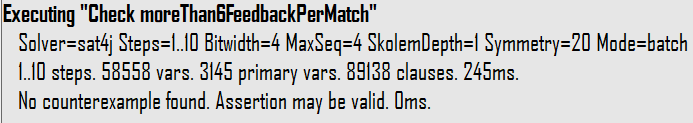
\includegraphics[width=0.8\textwidth]{Images/AlloyModel_images/moreThan6FeedbackPerMatch.png}
    \caption{moreThan6FeedbackPerMatch}
    \label{fig:figure2}
\end{figure}
Assertion to check that the maximum number of feedback linked to a match cannot be over 6 (3 possible states and 2 directions for each).

%------------------------------------------------
\clearpage

\subsubsection{State Machine for Successful Match Evolution}
\begin{lstlisting}
pred SuccessfulMatchEvolution [m : Match] {
	//Student
	#Student = 1
	#Competence = 0
	//Company
	#Company = 1
	#InternshipAdv = 1
	//S&C
	#Recommendation = 0
	#Match = 1
	#Feedback = 0
	MatchProgress[m]
}

run SuccessfulMatchEvolution for 6
\end{lstlisting}

\begin{figure}[h]
    \centering
    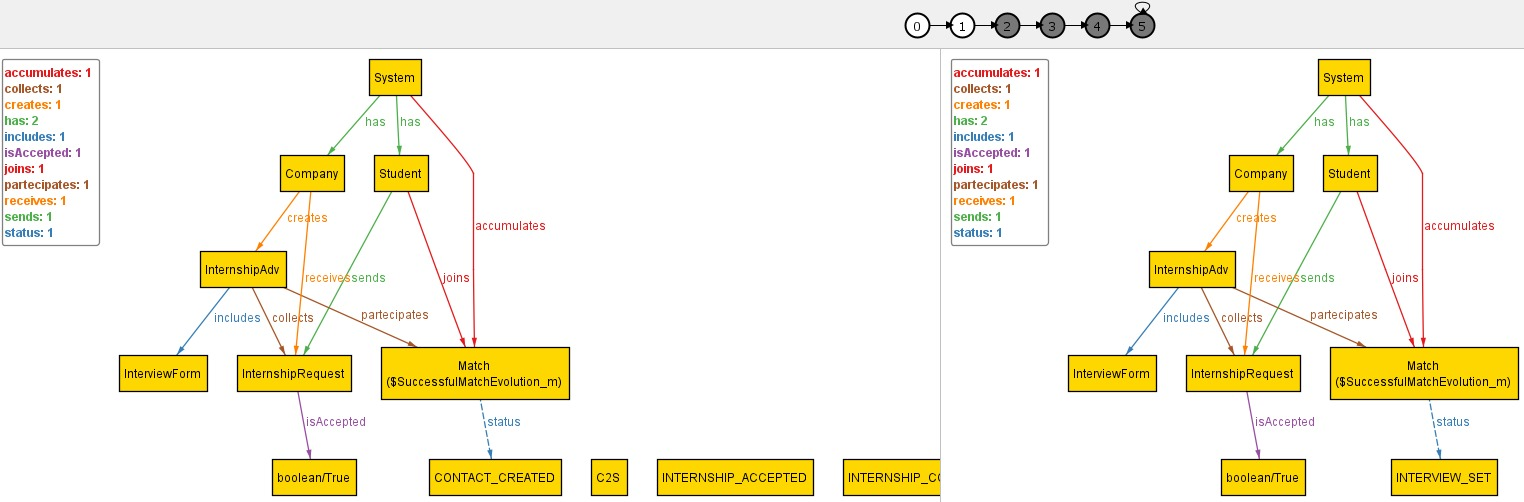
\includegraphics[width=1\textwidth]{Images/AlloyModel_images/SuccessfulMatchEvolution[0-1].png}
    \caption{SuccessfulMatchEvolution[0-1]}
    \label{fig:figure2}
\end{figure}
\begin{figure}[h]
    \centering
    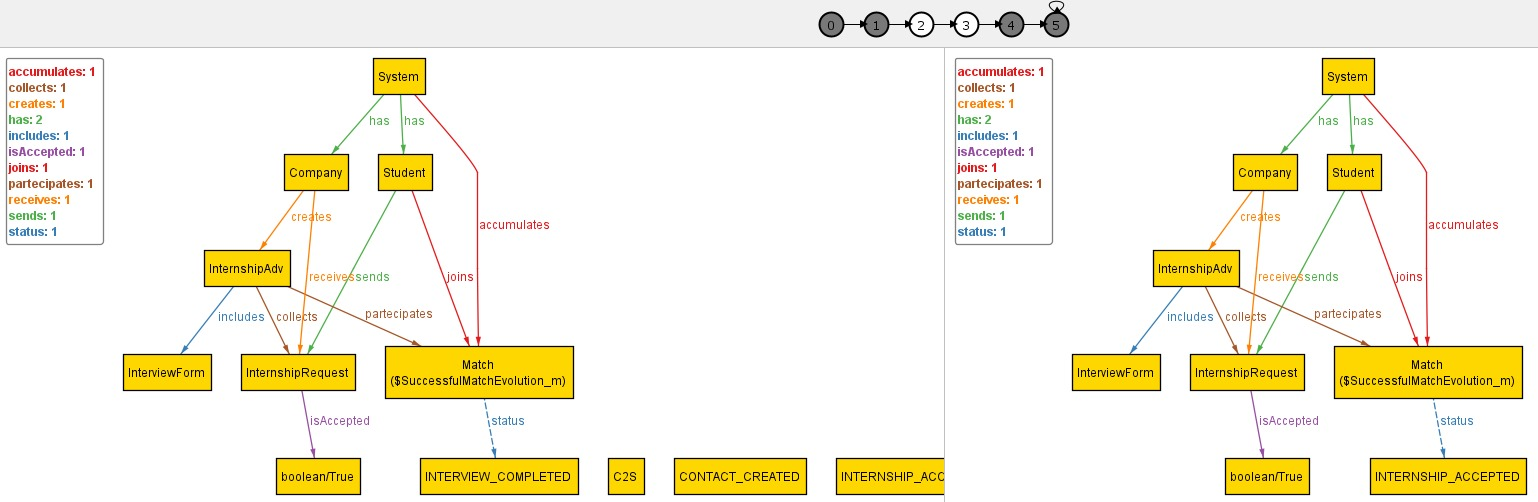
\includegraphics[width=1\textwidth]{Images/AlloyModel_images/SuccessfulMatchEvolution[2-3].png}
    \caption{SuccessfulMatchEvolution[2-3]}
    \label{fig:figure2}
\end{figure}
\begin{figure}[h]
    \centering
    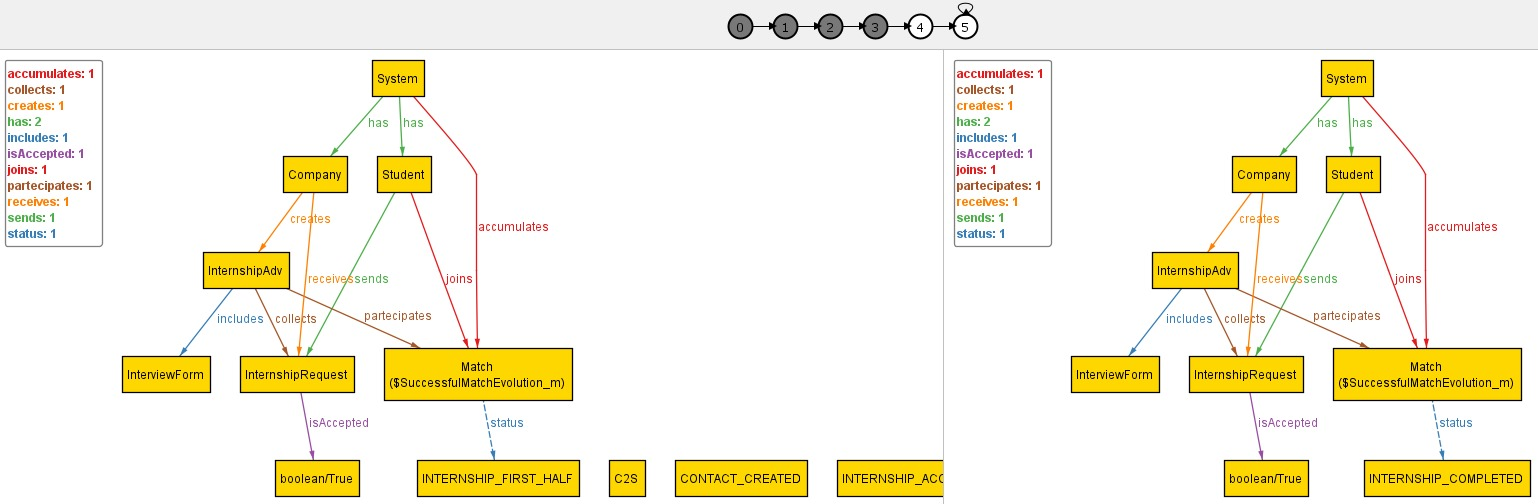
\includegraphics[width=1\textwidth]{Images/AlloyModel_images/SuccessfulMatchEvolution[4-4].png}
    \caption{SuccessfulMatchEvolution[4-4]}
    \label{fig:figure2}
\end{figure}
State machine that describes the behavior of the match Status in a Successful Match Situation (Interview lead to an Internship).

%------------------------------------------------
\clearpage

\subsubsection{State Machine for Unsuccessful Match Evolution}
\begin{lstlisting}
pred UnsuccessfulMatchEvolution [m : Match] {
	//Student
	#Student = 1
	#Competence = 0
	//Company
	#Company = 1
	#InternshipAdv = 1
	//S&C
	#Recommendation = 0
	#Match = 1
	#Feedback = 0
	MatchProgressDeclined[m]
}

run UnsuccessfulMatchEvolution for 6
\end{lstlisting}

\begin{figure}[h]
    \centering
    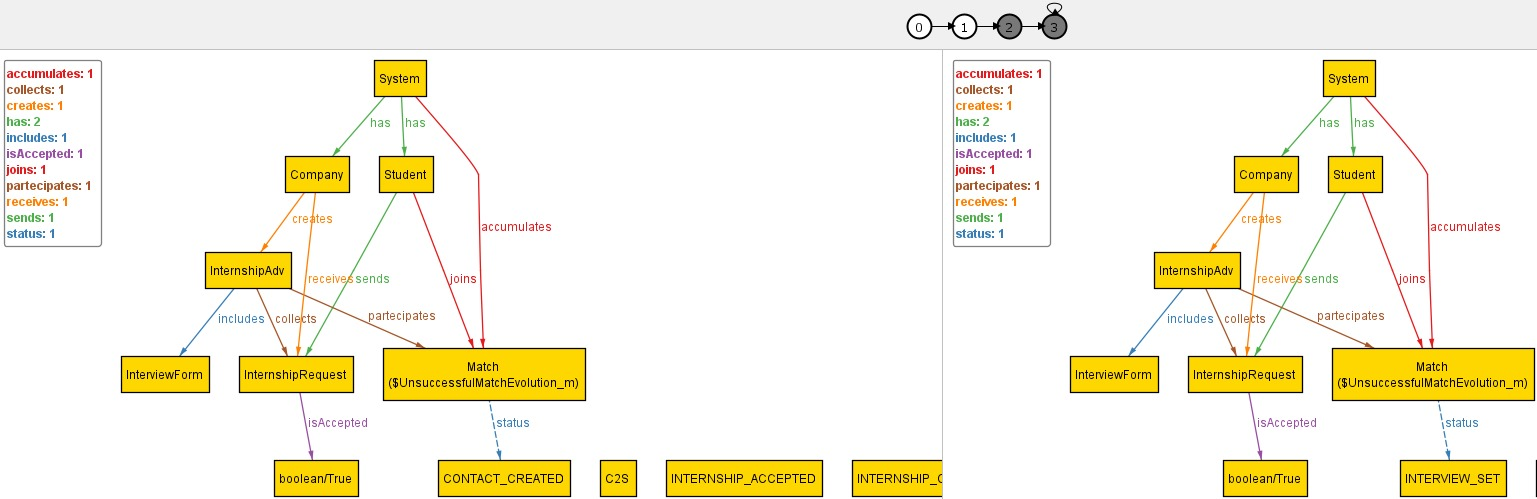
\includegraphics[width=0.85\textwidth]{Images/AlloyModel_images/UnsuccessfulMatchEvolution[0-1].png}
\caption{UnsuccessfulMatchEvolution[0-1]}
    \label{fig:figure2}
\end{figure}
\begin{figure}[h]
    \centering
    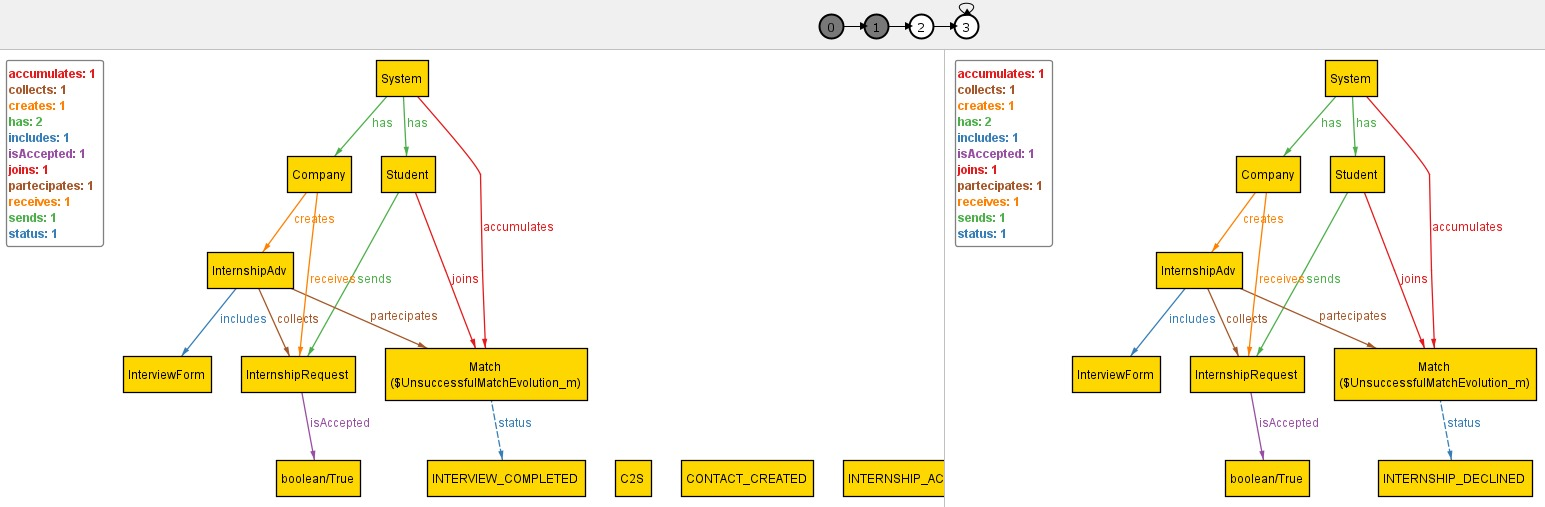
\includegraphics[width=0.85\textwidth]{Images/AlloyModel_images/UnsuccessfulMatchEvolution[2-2].png}
    \caption{UnsuccessfulMatchEvolution[2-2]}
    \label{fig:figure2}
\end{figure}
State machine that describes the behavior of the match Status in a Unsuccessful Match Situation (Interview do not lead to an Internship).

%------------------------------------------------
\clearpage

\subsubsection{Big World}
\begin{lstlisting}
pred BigWorld {
	//Student
	#Student = 2
	#Competence = 1
	//Company
	#Company = 2
	#InternshipAdv = 1
	//S&C
	#Recommendation = 0
	#Match = 2
	#Feedback = 1
}

run BigWorld for 6
\end{lstlisting}

\begin{figure}[h]
    \centering
    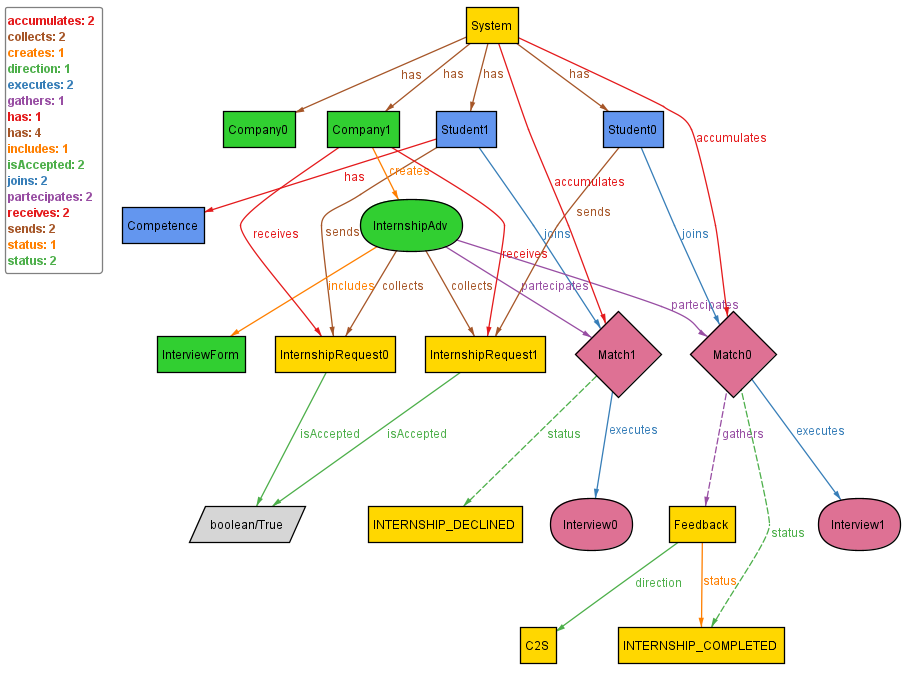
\includegraphics[width=1\textwidth]{Images/AlloyModel_images/BigWorld.png}
    \caption{BigWorld}
    \label{fig:figure2}
\end{figure}
Example of a more complex structure with multiple Students and Companies, which interact with each other creating InternshipRequest, Match and writing Feedback.


\pagebreak
\chapter{Effort Spent}
This is an overview of the number of hours spent on each chapter. Most of the work was done in pairs. However, an approximation of the number of hours contributed by each member is provided.
\begin{table}[]
    \centering
    \begin{tabular}{|c|c|c|}
        \hline
        - & \textbf{Irene Lo Presti} & \textbf{Matteo Lussana} \\\hline
        General Design of the project& 4h & 4h \\\hline
        Introduction & 5h & 3h \\\hline
        Overall Description & 20h & 19h \\\hline
        Specific Requirements & 14h & 16h \\\hline
        Formal Analysis& 20h & 21h \\\hline
    \end{tabular}
\end{table}

\pagebreak
\chapter{References}
\section{References}
\begin{itemize}
    \item Specification document: Assignment RDD AY 2024-2025. 
    \item Slides of the course "Software Engineering 2" held at Politecnico di Milano by Professor Rossi (a.y. 2024-25).
    \item Some definitions from the Definitions, Acronyms, Abbreviations section are taken from researches done on the Internet.
\end{itemize}
\section{Used Tools}
\begin{itemize}
    \item GitHub for project versioning and sharing.
    \item \LaTeX\space and \textit{Overleaf} as editor for writing this document.
    \item \textit{draw.io} for diagrams design.
    \item \textit{Notion} for collaborative organisation.
\end{itemize}
\pagebreak
\listoffigures
\listoftables




\end{document}
